\section{Test Results}
We test proposed techinque using the use cased explained in the previouse section.

\subsection{Verification of Results}

From Figure~\ref{fig:TestResults:distance0} we see that the simulation compared to the real-world results from Figure \ref{} is a close match. 
We see the same stop and go behavior as a results from traffic lights, and the arrival times are also a close match. 
If we compare the driving speed of the simulation show in Figure \ref{fig:TestResults:speed0} with the real-world data from Figure \ref{} we see that in most cases the vehicles are either driving at the maximum speed, or they are at a full stop. 
This behavior on the two graphs are almost identical and consistent with the stop and go behavior caused by traffic lights. 
Figure \ref{} shows the distance to a traffic light where each vehicles makes a stop. 
All the blue dots are vehicles that only have a single stop, red squares have two stops and yellow triangles have 3 stops.
The traffic light for this figure is the first junctions driving from Vesterbro. See Figure \ref{fig:Introduction:hobro}. The Figure \ref{} show the real-world data from the same traffic light. 
%TODO: when we have something to compare with

\begin{figure}[htb]
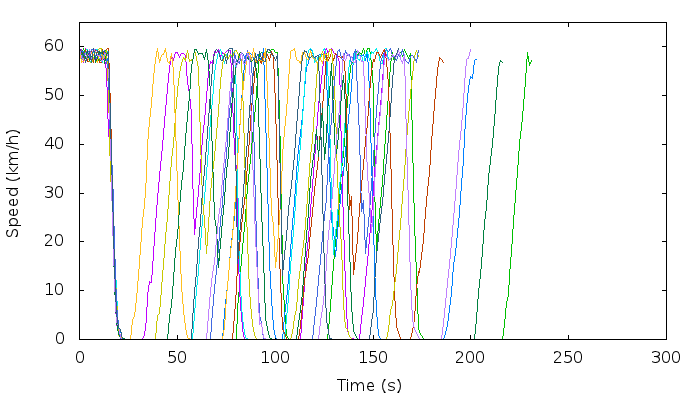
\includegraphics[width=0.5\textwidth]{images/tp0/speed0.png}
\caption{Speed graph}
\label{fig:TestResults:speed0}
\end{figure}

\begin{figure}[htb]
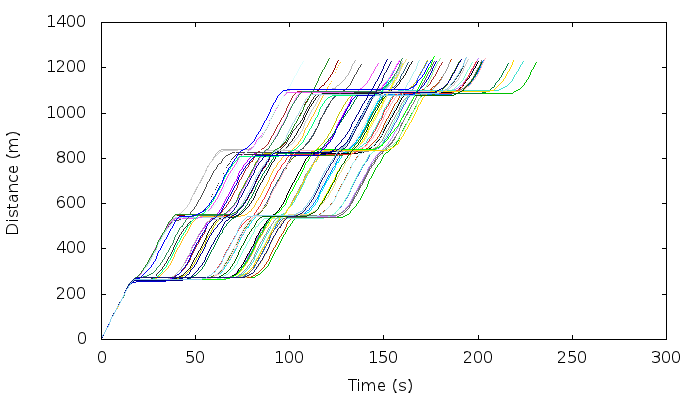
\includegraphics[width=0.5\textwidth]{images/tp0/distance0.png}
\caption{Distance graph}
\label{fig:TestResults:distance0}
\end{figure}

%
\begin{figure}
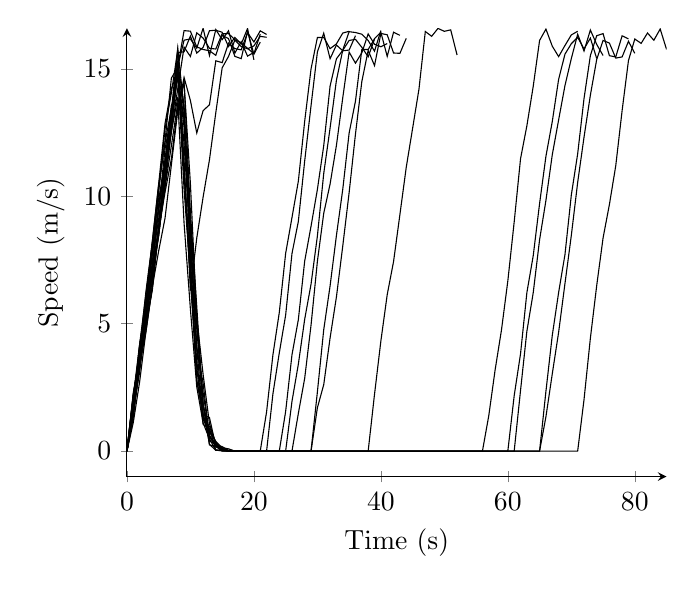
\begin{tikzpicture}
\begin{axis}[
legend style={anchor=west},
axis x line=bottom,
axis y line=left,
ymin=-1,
xlabel=Time (s),
ylabel=Speed (m/s),
]
\addplot[] coordinates {
(0, 0.0)
(1, 1.69655878999)
(2, 3.67956839706)
(3, 5.19272490987)
(4, 7.20356419508)
(5, 8.5737242637)
(6, 10.7899166882)
(7, 12.5081667572)
(8, 14.2099448128)
(9, 15.8518676442)
(10, 15.4860138311)
(11, 16.4121611704)
(12, 16.2075640619)
(13, 15.805771308)
(14, 15.7770029409)
(15, 16.376577111)
(16, 16.379913727)
(17, 16.1471423445)
(18, 16.0138479285)
(19, 15.8056926081)
(20, 15.5941200483)
(21, 16.3613227376)
};
\addplot[] coordinates {
(0, 0.0)
(1, 2.21121398936)
(2, 3.59285451821)
(3, 5.45790431643)
(4, 7.08020272548)
(5, 9.53823663498)
(6, 11.4596679897)
(7, 13.3623035229)
(8, 14.8760363605)
(9, 12.0485909913)
(10, 8.1243544415)
(11, 4.04465906846)
(12, 1.29806627542)
(13, 0.965862562495)
(14, 0.318337276114)
(15, 0.0815088310026)
(16, 0.0203345879742)
(17, 0.0)
(18, 0.0)
(19, 0.0)
(20, 0.0)
(21, 0.0)
(22, 0.0)
(23, 0.0)
(24, 0.0)
(25, 1.55413603643)
(26, 3.77907186659)
(27, 5.15578950755)
(28, 7.45418968872)
(29, 8.82250386494)
(30, 10.2651877131)
(31, 11.9845689784)
(32, 14.3253558327)
(33, 15.3939306363)
(34, 15.7255389416)
(35, 16.1136710649)
(36, 16.1571932173)
(37, 15.8447128613)
(38, 15.4723728657)
(39, 16.1609261253)
};
\addplot[] coordinates {
(0, 0.0)
(1, 1.57429128769)
(2, 3.53650107689)
(3, 4.99217562319)
(4, 6.44208426325)
(5, 7.85435972153)
(6, 9.13540175854)
(7, 11.2277544598)
(8, 13.3369616038)
(9, 14.6629914441)
(10, 13.7562936201)
(11, 12.4838164913)
(12, 13.3583665095)
(13, 13.5890204041)
(14, 15.3150675343)
(15, 15.2439689759)
(16, 16.0071006542)
(17, 15.793851726)
(18, 15.7440448308)
(19, 16.4194145001)
(20, 16.0551274081)
(21, 16.4913308166)
(22, 16.3489043325)
};
\addplot[] coordinates {
(0, 0.0)
(1, 1.59891751121)
(2, 3.98457542112)
(3, 6.27387736363)
(4, 8.19742514482)
(5, 10.4383861724)
(6, 12.0936067899)
(7, 13.4403211308)
(8, 14.8479898922)
(9, 10.9908702879)
(10, 7.30053526354)
(11, 3.29626058053)
(12, 1.04572542945)
(13, 0.883870550075)
(14, 0.0496195717564)
(15, 0.0259550926758)
(16, 0.0161643831833)
(17, 0.0)
(18, 0.0)
(19, 0.0)
(20, 0.0)
(21, 0.0)
(22, 0.0)
(23, 0.0)
(24, 0.0)
(25, 0.0)
(26, 0.0)
(27, 0.0)
(28, 0.0)
(29, 0.0)
(30, 0.0)
(31, 0.0)
(32, 0.0)
(33, 0.0)
(34, 0.0)
(35, 0.0)
(36, 0.0)
(37, 0.0)
(38, 0.0)
(39, 2.22701815801)
(40, 4.31829619425)
(41, 6.13777380728)
(42, 7.43947288312)
(43, 9.28266234085)
(44, 11.1397831561)
(45, 12.6635801216)
(46, 14.2016706953)
(47, 16.4656396166)
(48, 16.2764431518)
(49, 16.5862954565)
(50, 16.4718890772)
(51, 16.5296137568)
(52, 15.5456225908)
};
\addplot[] coordinates {
(0, 0.0)
(1, 1.44117465738)
(2, 3.44338031864)
(3, 5.28968274622)
(4, 7.29384729726)
(5, 9.67850462795)
(6, 11.1405541011)
(7, 12.6398144106)
(8, 14.9880648046)
(9, 13.3379256958)
(10, 7.78188122213)
(11, 5.1435470078)
(12, 1.86518108958)
(13, 0.242447056624)
(14, 0.187500411133)
(15, 0.0139345132501)
(16, 0.0)
(17, 0.0)
(18, 0.0)
(19, 0.0)
(20, 0.0)
(21, 0.0)
(22, 1.5402096021)
(23, 3.78246421518)
(24, 5.43688386446)
(25, 7.7562591451)
(26, 9.16652720276)
(27, 10.5898654248)
(28, 12.9424510061)
(29, 14.9969998465)
(30, 16.2278432352)
(31, 16.2351880036)
(32, 15.7912144583)
(33, 15.9791797187)
(34, 16.4046871013)
(35, 16.4727939988)
};
\addplot[] coordinates {
(0, 0.0)
(1, 2.12616742007)
(2, 4.19329186872)
(3, 5.6919135229)
(4, 7.89838829078)
(5, 10.2796010577)
(6, 12.1599819956)
(7, 14.6357143813)
(8, 15.0528237228)
(9, 11.4158128506)
(10, 6.297614139)
(11, 8.35899559487)
(12, 9.96607545993)
(13, 11.432352401)
(14, 13.2800165118)
(15, 15.0379895419)
(16, 15.4857963213)
(17, 16.1255716614)
(18, 15.8771209058)
(19, 15.7861428542)
(20, 15.9017509198)
(21, 16.2739378924)
(22, 16.2391567355)
};
\addplot[] coordinates {
(0, 0.0)
(1, 1.93305703113)
(2, 4.13554966013)
(3, 5.72500893526)
(4, 8.0593960773)
(5, 9.46967692056)
(6, 11.854418639)
(7, 13.1735351184)
(8, 15.6387967503)
(9, 15.669845863)
(10, 16.2888681309)
(11, 15.6172210126)
(12, 15.842290706)
(13, 16.4945108891)
(14, 16.5160755018)
(15, 16.4343506109)
(16, 15.8733656333)
(17, 16.2335178043)
(18, 15.9711069616)
(19, 16.5846852335)
(20, 15.3518956352)
};
\addplot[] coordinates {
(0, 0.0)
(1, 1.72800719243)
(2, 3.55822897458)
(3, 5.55445920385)
(4, 7.80072680674)
(5, 10.1552350406)
(6, 12.6490986621)
(7, 14.0492980054)
(8, 15.7339862424)
(9, 11.087762116)
(10, 7.23641608203)
(11, 2.78237483288)
(12, 1.43614198184)
(13, 0.394618942235)
(14, 0.265801609592)
(15, 0.0420118674928)
(16, 0.011768430675)
(17, 0.0)
(18, 0.0)
(19, 0.0)
(20, 0.0)
(21, 0.0)
(22, 0.0)
(23, 0.0)
(24, 0.0)
(25, 0.0)
(26, 0.0)
(27, 0.0)
(28, 0.0)
(29, 0.0)
(30, 0.0)
(31, 0.0)
(32, 0.0)
(33, 0.0)
(34, 0.0)
(35, 0.0)
(36, 0.0)
(37, 0.0)
(38, 0.0)
(39, 0.0)
(40, 0.0)
(41, 0.0)
(42, 0.0)
(43, 0.0)
(44, 0.0)
(45, 0.0)
(46, 0.0)
(47, 0.0)
(48, 0.0)
(49, 0.0)
(50, 0.0)
(51, 0.0)
(52, 0.0)
(53, 0.0)
(54, 0.0)
(55, 0.0)
(56, 0.0)
(57, 1.3926015349)
(58, 3.18965922255)
(59, 4.7542434599)
(60, 6.68003495724)
(61, 8.99055800546)
(62, 11.4714384041)
(63, 12.7666285957)
(64, 14.3153023391)
(65, 16.1122029411)
(66, 16.559530771)
(67, 15.8895344371)
(68, 15.4795046508)
(69, 15.9167218118)
(70, 16.330392858)
(71, 16.4747433422)
};
\addplot[] coordinates {
(0, 0.0)
(1, 2.15391133737)
(2, 3.92069633061)
(3, 5.68047448178)
(4, 7.01535401953)
(5, 8.43687932327)
(6, 10.6935469003)
(7, 12.7973568795)
(8, 14.7339270296)
(9, 13.0211991519)
(10, 8.67103513938)
(11, 4.11339048306)
(12, 2.2963351297)
(13, 0.580072811148)
(14, 0.282998586036)
(15, 0.0863961507886)
(16, 0.0)
(17, 0.0)
(18, 0.0)
(19, 0.0)
(20, 0.0)
(21, 0.0)
(22, 0.0)
(23, 0.0)
(24, 0.0)
(25, 0.0)
(26, 0.0)
(27, 0.0)
(28, 0.0)
(29, 0.0)
(30, 0.0)
(31, 0.0)
(32, 0.0)
(33, 0.0)
(34, 0.0)
(35, 0.0)
(36, 0.0)
(37, 0.0)
(38, 0.0)
(39, 0.0)
(40, 0.0)
(41, 0.0)
(42, 0.0)
(43, 0.0)
(44, 0.0)
(45, 0.0)
(46, 0.0)
(47, 0.0)
(48, 0.0)
(49, 0.0)
(50, 0.0)
(51, 0.0)
(52, 0.0)
(53, 0.0)
(54, 0.0)
(55, 0.0)
(56, 0.0)
(57, 0.0)
(58, 0.0)
(59, 0.0)
(60, 0.0)
(61, 0.0)
(62, 0.0)
(63, 0.0)
(64, 0.0)
(65, 0.0)
(66, 0.0)
(67, 0.0)
(68, 0.0)
(69, 0.0)
(70, 0.0)
(71, 0.0)
(72, 2.01908573479)
(73, 4.42585163808)
(74, 6.49724935094)
(75, 8.36174359778)
(76, 9.67761302018)
(77, 11.1979801283)
(78, 13.3601725296)
(79, 15.3238696061)
(80, 16.1702353035)
(81, 15.9989677579)
(82, 16.4057737105)
(83, 16.1208111173)
(84, 16.5637219947)
(85, 15.7610954609)
};
\addplot[] coordinates {
(0, 0.0)
(1, 1.56946584146)
(2, 3.09415850206)
(3, 5.13459491602)
(4, 6.70768423559)
(5, 8.45885561605)
(6, 10.6505276111)
(7, 13.1024183906)
(8, 15.2725959348)
(9, 13.5691848483)
(10, 8.79965043157)
(11, 5.29816334608)
(12, 1.77933855823)
(13, 0.622337701857)
(14, 0.233352224777)
(15, 0.176862404631)
(16, 0.0194313604896)
(17, 0.0)
(18, 0.0)
(19, 0.0)
(20, 0.0)
(21, 0.0)
(22, 0.0)
(23, 0.0)
(24, 0.0)
(25, 0.0)
(26, 1.95257699525)
(27, 3.4067007812)
(28, 5.17198963236)
(29, 6.5479420044)
(30, 8.43751423468)
(31, 10.891402156)
(32, 12.6752913179)
(33, 14.5514645832)
(34, 15.7399044552)
(35, 16.4574820848)
(36, 16.4251046459)
(37, 16.3598376629)
(38, 16.1124643348)
(39, 15.6938809124)
(40, 16.5001951495)
};
\addplot[] coordinates {
(0, 0.0)
(1, 1.76217175409)
(2, 3.95900752424)
(3, 5.88440275606)
(4, 8.238239036)
(5, 10.4874022488)
(6, 12.8510501594)
(7, 14.2197145952)
(8, 14.8875235286)
(9, 10.2819409787)
(10, 6.85276609781)
(11, 2.75159340453)
(12, 1.43282266635)
(13, 0.61206581378)
(14, 0.166196718036)
(15, 0.0960943362038)
(16, 0.0)
(17, 0.0)
(18, 0.0)
(19, 0.0)
(20, 0.0)
(21, 0.0)
(22, 0.0)
(23, 0.0)
(24, 0.0)
(25, 0.0)
(26, 0.0)
(27, 0.0)
(28, 0.0)
(29, 0.0)
(30, 0.0)
(31, 0.0)
(32, 0.0)
(33, 0.0)
(34, 0.0)
(35, 0.0)
(36, 0.0)
(37, 0.0)
(38, 0.0)
(39, 0.0)
(40, 0.0)
(41, 0.0)
(42, 0.0)
(43, 0.0)
(44, 0.0)
(45, 0.0)
(46, 0.0)
(47, 0.0)
(48, 0.0)
(49, 0.0)
(50, 0.0)
(51, 0.0)
(52, 0.0)
(53, 0.0)
(54, 0.0)
(55, 0.0)
(56, 0.0)
(57, 0.0)
(58, 0.0)
(59, 0.0)
(60, 0.0)
(61, 2.17250207817)
(62, 3.81653779303)
(63, 6.22125260328)
(64, 7.66564355261)
(65, 9.71165935218)
(66, 11.5674470877)
(67, 12.9311783827)
(68, 14.5882285229)
(69, 15.5764424524)
(70, 15.9871104351)
(71, 16.2367633803)
(72, 15.7811718294)
(73, 16.2054076054)
(74, 15.4049100628)
};
\addplot[] coordinates {
(0, 0.0)
(1, 2.28535288596)
(2, 3.70210856199)
(3, 5.52483096719)
(4, 7.71647389338)
(5, 9.45676035044)
(6, 11.2365432421)
(7, 12.5545747174)
(8, 13.8425897987)
(9, 13.2098117887)
(10, 7.46539523987)
(11, 4.01294297319)
(12, 2.66552671691)
(13, 0.537530884295)
(14, 0.227326585301)
(15, 0.0376341870259)
(16, 0.0135643362328)
(17, 0.0)
(18, 0.0)
(19, 0.0)
(20, 0.0)
(21, 0.0)
(22, 0.0)
(23, 0.0)
(24, 0.0)
(25, 0.0)
(26, 0.0)
(27, 0.0)
(28, 0.0)
(29, 0.0)
(30, 0.0)
(31, 0.0)
(32, 0.0)
(33, 0.0)
(34, 0.0)
(35, 0.0)
(36, 0.0)
(37, 0.0)
(38, 0.0)
(39, 0.0)
(40, 0.0)
(41, 0.0)
(42, 0.0)
(43, 0.0)
(44, 0.0)
(45, 0.0)
(46, 0.0)
(47, 0.0)
(48, 0.0)
(49, 0.0)
(50, 0.0)
(51, 0.0)
(52, 0.0)
(53, 0.0)
(54, 0.0)
(55, 0.0)
(56, 0.0)
(57, 0.0)
(58, 0.0)
(59, 0.0)
(60, 0.0)
(61, 0.0)
(62, 2.37832577695)
(63, 4.70544832642)
(64, 6.21493324608)
(65, 8.29173558566)
(66, 9.83625754452)
(67, 11.6286560611)
(68, 12.9952759296)
(69, 14.3451326288)
(70, 15.4013464038)
(71, 16.3579293678)
(72, 15.698878589)
(73, 16.5228580011)
(74, 15.9589924782)
(75, 15.5234330648)
};
\addplot[] coordinates {
(0, 0.0)
(1, 1.12030713827)
(2, 2.71622399516)
(3, 4.70346487281)
(4, 6.47660057156)
(5, 8.80941922202)
(6, 10.9377210189)
(7, 13.3359793443)
(8, 15.8064862106)
(9, 13.4117578671)
(10, 9.08639131299)
(11, 5.16091423356)
(12, 1.41781840424)
(13, 1.31776415859)
(14, 0.185346760293)
(15, 0.0)
(16, 0.0)
(17, 0.0)
(18, 0.0)
(19, 0.0)
(20, 0.0)
(21, 0.0)
(22, 0.0)
(23, 0.0)
(24, 0.0)
(25, 0.0)
(26, 0.0)
(27, 0.0)
(28, 0.0)
(29, 0.0)
(30, 2.3181127882)
(31, 4.76290456543)
(32, 6.48089444294)
(33, 8.45874933992)
(34, 10.2764157305)
(35, 12.479780346)
(36, 13.732967882)
(37, 15.763519952)
(38, 15.7560555369)
(39, 16.183223447)
(40, 16.4315775002)
(41, 15.4895587344)
(42, 16.4357821468)
(43, 16.3152276867)
};
\addplot[] coordinates {
(0, 0.0)
(1, 1.71211540815)
(2, 3.4546336325)
(3, 5.1277389942)
(4, 6.98726067058)
(5, 8.50697032613)
(6, 10.3430498377)
(7, 11.9826646519)
(8, 13.6399594214)
(9, 14.4800770819)
(10, 9.35702731021)
(11, 5.67568528481)
(12, 1.81795053343)
(13, 0.800644009561)
(14, 0.381808491778)
(15, 0.130464529991)
(16, 0.088226441567)
(17, 0.0)
(18, 0.0)
(19, 0.0)
(20, 0.0)
(21, 0.0)
(22, 0.0)
(23, 0.0)
(24, 0.0)
(25, 0.0)
(26, 0.0)
(27, 0.0)
(28, 0.0)
(29, 0.0)
(30, 0.0)
(31, 0.0)
(32, 0.0)
(33, 0.0)
(34, 0.0)
(35, 0.0)
(36, 0.0)
(37, 0.0)
(38, 0.0)
(39, 0.0)
(40, 0.0)
(41, 0.0)
(42, 0.0)
(43, 0.0)
(44, 0.0)
(45, 0.0)
(46, 0.0)
(47, 0.0)
(48, 0.0)
(49, 0.0)
(50, 0.0)
(51, 0.0)
(52, 0.0)
(53, 0.0)
(54, 0.0)
(55, 0.0)
(56, 0.0)
(57, 0.0)
(58, 0.0)
(59, 0.0)
(60, 0.0)
(61, 0.0)
(62, 0.0)
(63, 0.0)
(64, 0.0)
(65, 0.0)
(66, 2.34437234176)
(67, 4.54136070621)
(68, 6.22095976694)
(69, 7.71238190442)
(70, 10.0488391911)
(71, 11.666006748)
(72, 13.8343140256)
(73, 15.5194134946)
(74, 16.2991600754)
(75, 16.3816599612)
(76, 15.5161994774)
(77, 15.4667910174)
(78, 16.2960973914)
(79, 16.1748927208)
};
\addplot[] coordinates {
(0, 0.0)
(1, 1.7559286466)
(2, 4.17839807138)
(3, 6.15744372713)
(4, 8.1321092046)
(5, 9.90082604752)
(6, 11.2672997007)
(7, 13.5754609277)
(8, 13.8556722044)
(9, 8.94275931581)
(10, 5.56644422776)
(11, 2.51877664067)
(12, 1.10664772248)
(13, 0.478721600681)
(14, 0.0342486046173)
(15, 0.0105822033696)
(16, 0.0)
(17, 0.0)
(18, 0.0)
(19, 0.0)
(20, 0.0)
(21, 0.0)
(22, 0.0)
(23, 0.0)
(24, 0.0)
(25, 0.0)
(26, 0.0)
(27, 1.47661198202)
(28, 2.85346646622)
(29, 4.94034460982)
(30, 7.44019067384)
(31, 9.33155797207)
(32, 10.4774459202)
(33, 11.9960673661)
(34, 13.8683061093)
(35, 15.6580634917)
(36, 15.222881409)
(37, 15.6295543376)
(38, 16.3704201101)
(39, 15.9641190176)
(40, 15.8681369639)
(41, 15.9908659121)
};
\addplot[] coordinates {
(0, 0.0)
(1, 2.1931301101)
(2, 3.71601672668)
(3, 5.91884335241)
(4, 7.17229086003)
(5, 8.77609472605)
(6, 11.2683350412)
(7, 13.0174985688)
(8, 14.7399002651)
(9, 12.7181939845)
(10, 8.05154222418)
(11, 4.82021886674)
(12, 1.78309993627)
(13, 0.26462377161)
(14, 0.0292041260898)
(15, 0.0203721756787)
(16, 0.0)
(17, 0.0)
(18, 0.0)
(19, 0.0)
(20, 0.0)
(21, 0.0)
(22, 0.0)
(23, 0.0)
(24, 0.0)
(25, 0.0)
(26, 0.0)
(27, 0.0)
(28, 0.0)
(29, 0.0)
(30, 0.0)
(31, 0.0)
(32, 0.0)
(33, 0.0)
(34, 0.0)
(35, 0.0)
(36, 0.0)
(37, 0.0)
(38, 0.0)
(39, 0.0)
(40, 0.0)
(41, 0.0)
(42, 0.0)
(43, 0.0)
(44, 0.0)
(45, 0.0)
(46, 0.0)
(47, 0.0)
(48, 0.0)
(49, 0.0)
(50, 0.0)
(51, 0.0)
(52, 0.0)
(53, 0.0)
(54, 0.0)
(55, 0.0)
(56, 0.0)
(57, 0.0)
(58, 0.0)
(59, 0.0)
(60, 0.0)
(61, 0.0)
(62, 0.0)
(63, 0.0)
(64, 0.0)
(65, 0.0)
(66, 1.34787296818)
(67, 3.03080347134)
(68, 4.66036999889)
(69, 6.57794601197)
(70, 8.46123299445)
(71, 10.5417028748)
(72, 12.3173160938)
(73, 13.9664611532)
(74, 15.3699047092)
(75, 16.1149546533)
(76, 16.0092375482)
(77, 15.4218084563)
(78, 15.4672602017)
(79, 16.0790583121)
(80, 15.6084543076)
};
\addplot[] coordinates {
(0, 0.0)
(1, 1.33937796112)
(2, 3.37042703875)
(3, 4.68622733228)
(4, 6.44059778453)
(5, 8.82718025707)
(6, 11.2937324727)
(7, 13.2140702088)
(8, 14.7871380675)
(9, 10.9154684694)
(10, 6.6019721695)
(11, 3.56478113788)
(12, 1.24447726752)
(13, 0.736013935905)
(14, 0.363874127111)
(15, 0.0521636831607)
(16, 0.0372039301713)
(17, 0.0)
(18, 0.0)
(19, 0.0)
(20, 0.0)
(21, 0.0)
(22, 0.0)
(23, 0.0)
(24, 0.0)
(25, 0.0)
(26, 0.0)
(27, 0.0)
(28, 0.0)
(29, 0.0)
(30, 1.69885161612)
(31, 2.60542856077)
(32, 4.43813120639)
(33, 6.05007122226)
(34, 8.05048696099)
(35, 10.1402692676)
(36, 12.4421272807)
(37, 14.4993225999)
(38, 15.7240861325)
(39, 15.1270575308)
(40, 16.3888795129)
(41, 16.336593481)
(42, 15.6224220142)
(43, 15.6076675653)
(44, 16.195384867)
};
\addplot[] coordinates {
(0, 0.0)
(1, 1.89841344021)
(2, 3.36315647204)
(3, 4.96827411989)
(4, 7.44419015595)
(5, 9.11606207519)
(6, 10.9405574974)
(7, 13.0638682193)
(8, 15.0902371138)
(9, 16.123774737)
(10, 16.1730267122)
(11, 15.8101402988)
(12, 16.5937052905)
(13, 15.5203149683)
(14, 16.5403290221)
(15, 16.1453285397)
(16, 16.4915013648)
(17, 15.6183031792)
(18, 16.0636116127)
(19, 15.4992142314)
(20, 15.6461470993)
};
\addplot[] coordinates {
(0, 0.0)
(1, 1.37464806001)
(2, 3.79522872769)
(3, 5.47972515487)
(4, 6.85412846651)
(5, 8.75942654558)
(6, 10.3674478998)
(7, 12.5815865429)
(8, 15.0694890399)
(9, 16.5003676744)
(10, 16.4764948198)
(11, 15.861284025)
(12, 15.7603240589)
(13, 15.7101096489)
(14, 15.5293914801)
(15, 16.3106130159)
(16, 16.1857220536)
(17, 15.4899544455)
(18, 15.3989865956)
(19, 16.4695790669)
(20, 15.5755449089)
(21, 16.0493228194)
};
\addplot[] coordinates {
(0, 0.0)
(1, 1.42226831173)
(2, 3.36769873073)
(3, 4.96723441145)
(4, 6.30851660564)
(5, 8.68287524703)
(6, 10.1535771968)
(7, 11.4578730206)
(8, 13.4757590172)
(9, 14.4400636634)
(10, 10.4859905255)
(11, 5.22558107515)
(12, 3.00656101795)
(13, 1.07455724449)
(14, 0.301068854158)
(15, 0.107670251233)
(16, 0.00725802285952)
(17, 0.0)
(18, 0.0)
(19, 0.0)
(20, 0.0)
(21, 0.0)
(22, 0.0)
(23, 2.2497973268)
(24, 3.85383423622)
(25, 5.33288294566)
(26, 7.75346572773)
(27, 9.00912920159)
(28, 11.382957116)
(29, 13.5506748891)
(30, 15.6589209466)
(31, 16.3957776554)
(32, 15.3957433538)
(33, 15.9344617213)
(34, 15.7066923575)
(35, 15.7381369953)
(36, 16.2999265184)
};

\end{axis}
\end{tikzpicture}
\label{tik:speed:0:53}
\caption{0 percent diving with GSC on route $53$}
\end{figure}

%
\begin{figure}
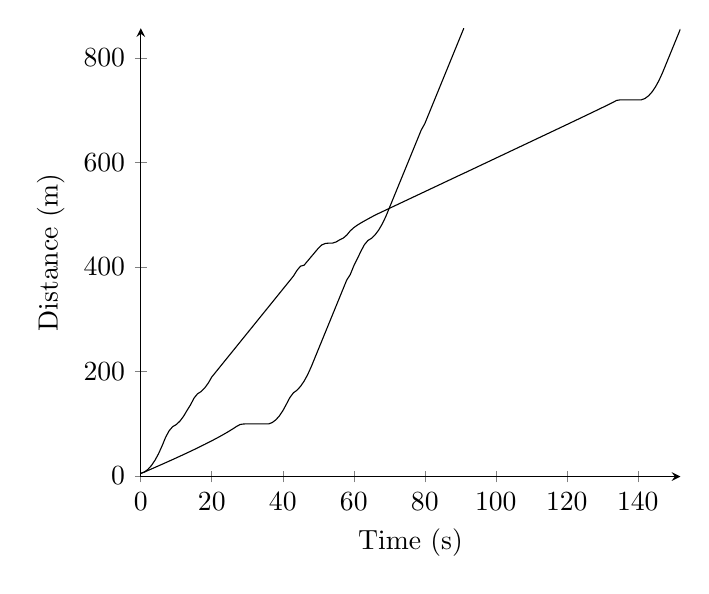
\begin{tikzpicture}
\begin{axis}[
legend style={anchor=west},
axis x line=bottom,
axis y line=left,
ymin=-1,
xlabel=Time (s),
ylabel=Distance (m),
]
\addplot[] coordinates {
(0, 5.1)
(1, 7.6)
(2, 10.551264739)
(3, 13.5148458518)
(4, 16.491720024)
(5, 19.4829705626)
(6, 22.4898024406)
(7, 25.5135599774)
(8, 28.555747716)
(9, 31.6180551961)
(10, 34.7023865031)
(11, 37.810895714)
(12, 40.9460296665)
(13, 44.1105798987)
(14, 47.3077461535)
(15, 50.5412145976)
(16, 53.8152549271)
(17, 57.1348419561)
(18, 60.5058092771)
(19, 63.9350454196)
(20, 67.4307470306)
(21, 71.0027496137)
(22, 74.6629653545)
(23, 78.4259712621)
(24, 82.309812202)
(25, 86.3371174595)
(26, 90.5366852977)
(27, 94.9457842613)
(28, 98.6044896023)
(29, 99.6320158223)
(30, 99.7193641886)
(31, 99.7193641886)
(32, 99.7193641886)
(33, 99.7193641886)
(34, 99.7193641886)
(35, 99.7193641886)
(36, 99.7193641886)
(37, 102.219364189)
(38, 107.219364189)
(39, 114.719364189)
(40, 124.719364189)
(41, 137.219364189)
(42, 150.125095958)
(43, 159.234657451)
(44, 164.142641251)
(45, 171.550625052)
(46, 181.458608852)
(47, 193.866592652)
(48, 208.774576453)
(49, 225.374576453)
(50, 241.974576453)
(51, 258.574576453)
(52, 275.174576453)
(53, 291.774576453)
(54, 308.374576453)
(55, 324.974576453)
(56, 341.574576453)
(57, 358.174576453)
(58, 374.774576453)
(59, 385.384576453)
(60, 401.984576453)
(61, 415.584576453)
(62, 429.92347141)
(63, 442.651450477)
(64, 450.734866052)
(65, 454.801722929)
(66, 461.368579805)
(67, 470.435436682)
(68, 482.002293558)
(69, 496.069150435)
(70, 512.636007311)
(71, 529.236007311)
(72, 545.836007311)
(73, 562.436007311)
(74, 578.936007311)
(75, 595.536007311)
(76, 612.136007311)
(77, 628.736007311)
(78, 645.336007311)
(79, 661.936007311)
(80, 674.076007311)
(81, 690.676007311)
(82, 707.276007311)
(83, 723.876007311)
(84, 740.476007311)
(85, 757.076007311)
(86, 773.676007311)
(87, 790.276007311)
(88, 806.876007311)
(89, 823.476007311)
(90, 840.076007311)
(91, 856.676007311)
};
\addplot[] coordinates {
(0, 5.1)
(1, 7.6)
(2, 12.6)
(3, 20.1)
(4, 30.1)
(5, 42.6)
(6, 57.6)
(7, 74.2)
(8, 86.6997297278)
(9, 94.5649106955)
(10, 98.4573862023)
(11, 104.849861709)
(12, 113.742337216)
(13, 125.134812723)
(14, 136.02728823)
(15, 149.039719459)
(16, 157.36882852)
(17, 161.634015209)
(18, 168.399201898)
(19, 177.664388587)
(20, 189.429575276)
(21, 197.822653454)
(22, 206.215777321)
(23, 214.6089514)
(24, 223.002180831)
(25, 231.39547148)
(26, 239.788830074)
(27, 248.182264361)
(28, 256.575783316)
(29, 264.969397389)
(30, 273.363118827)
(31, 281.756962071)
(32, 290.150944275)
(33, 298.545085976)
(34, 306.939411965)
(35, 315.333952455)
(36, 323.728744648)
(37, 332.123834879)
(38, 340.519281603)
(39, 348.915159643)
(40, 357.311566345)
(41, 365.708630755)
(42, 374.106527678)
(43, 382.505499944)
(44, 393.404472211)
(45, 401.495043603)
(46, 403.315921389)
(47, 411.406228382)
(48, 419.498021114)
(49, 427.592671136)
(50, 435.692811781)
(51, 442.135492037)
(52, 444.939362145)
(53, 445.562177829)
(54, 445.594416168)
(55, 447.718518537)
(56, 451.744076421)
(57, 455.010741568)
(58, 460.777406715)
(59, 468.983220762)
(60, 475.126173639)
(61, 479.98217806)
(62, 484.165440335)
(63, 488.045666837)
(64, 491.801513568)
(65, 495.508625682)
(66, 499.197053628)
(67, 502.398679294)
(68, 505.60038685)
(69, 508.802179833)
(70, 512.00406199)
(71, 515.206037288)
(72, 518.408109936)
(73, 521.610284397)
(74, 524.812565414)
(75, 528.014958028)
(76, 531.217467605)
(77, 534.420099859)
(78, 537.622860883)
(79, 540.825757181)
(80, 544.028795704)
(81, 547.231983886)
(82, 550.43532969)
(83, 553.638841654)
(84, 556.842528945)
(85, 560.046401418)
(86, 563.250469681)
(87, 566.454745168)
(88, 569.659240225)
(89, 572.863968196)
(90, 576.068943533)
(91, 579.17418191)
(92, 582.384466492)
(93, 585.594782946)
(94, 588.80513343)
(95, 592.015520299)
(96, 595.225946133)
(97, 598.436413761)
(98, 601.646926294)
(99, 604.857487159)
(100, 608.068100143)
(101, 611.278769439)
(102, 614.489499704)
(103, 617.700296122)
(104, 620.911164487)
(105, 624.122111289)
(106, 627.333143825)
(107, 630.54427033)
(108, 633.755500132)
(109, 636.966843838)
(110, 640.178313567)
(111, 643.389923225)
(112, 646.601688852)
(113, 649.81362905)
(114, 653.025765514)
(115, 656.238123711)
(116, 659.450733742)
(117, 662.663631452)
(118, 665.876859877)
(119, 669.090471166)
(120, 672.304426716)
(121, 675.540738148)
(122, 678.778922376)
(123, 682.019357719)
(124, 685.262533559)
(125, 688.509095201)
(126, 691.759912938)
(127, 695.016192554)
(128, 698.279660573)
(129, 701.552893549)
(130, 704.839949662)
(131, 708.147712295)
(132, 711.489214454)
(133, 714.894166483)
(134, 718.464164333)
(135, 719.59368241)
(136, 719.699074378)
(137, 719.699074378)
(138, 719.699074378)
(139, 719.699074378)
(140, 719.699074378)
(141, 719.699074378)
(142, 722.199074378)
(143, 727.199074378)
(144, 734.699074378)
(145, 744.699074378)
(146, 757.199074378)
(147, 772.199074378)
(148, 788.799074378)
(149, 805.399074378)
(150, 821.999074378)
(151, 838.599074378)
(152, 855.199074378)
};

\end{axis}
\end{tikzpicture}
\label{tik:distance:100:53}
\caption{100 percent diving with GSC on route $53$}
\end{figure}

%\begin{tikzpicture}\begin{axis}
};
\addplot+[ycomb] coordinates{
(216, 52.252945617)
(217, 10.2835247016)
(214, 16.2856718575)
(215, 4.51864792679)
(213, 28.3873548357)
(211, 11.189338998)
(264, 40.4878802965)
(218, 0)
(219, 22.2220848566)
(133, 0)
(132, 34.4508958132)
(131, 28.3594198907)
(130, 22.1385166496)
(137, 0)
(135, 4.50616611369)
(165, 16.2267027888)
(139, 28.285187868)
(225, 52.3061097447)
(25, 16.0530002679)
(26, 10.1475132786)
(167, 52.905635371)
(20, 4.06070836139)
(21, 0)
(95, 16.7780005237)
(28, 13.0397800766)
(29, 0)
(178, 40.1749084596)
(0, 0.887926285604)
(221, 11.0667215168)
(281, 28.1590830651)
(8, 0.879701275233)
(96, 10.9849476286)
(284, 33.0003184931)
(68, 7.55165507934)
(87, 7.01750211778)
(119, 22.4988880985)
(263, 0)
(121, 40.2128463437)
(261, 22.2161474214)
(124, 22.5816882433)
(265, 0)
(127, 34.5048855528)
(128, 0)
(129, 52.6828088003)
(269, 16.4398851063)
(268, 22.2261723856)
(183, 16.8024845352)
(59, 4.06105996166)
(58, 4.32362219439)
(55, 4.10269772145)
(54, 8.12141482104)
(227, 28.5551151413)
(50, 8.38010669551)
(53, 0)
(259, 22.7745844792)
(298, 0)
(296, 4.31694972892)
(297, 40.4553565181)
(294, 40.1480987865)
(295, 22.2334499586)
(292, 40.1264458833)
(293, 16.9100041831)
(291, 40.5409654352)
(199, 4.35555745706)
(66, 20.4512404622)
(134, 28.6189430663)
(194, 0)
(197, 10.2047254435)
(196, 21.1414626766)
(191, 16.8319208832)
(190, 22.5846717422)
(271, 0)
(273, 34.2295001485)
(111, 11.3590799416)
(275, 10.3466370086)
(276, 28.1627318956)
(82, 22.718673814)
(279, 16.198959792)
(81, 28.2427318469)
(86, 22.1371668922)
(175, 10.9783281237)
(84, 52.7044109674)
(85, 5.04021199249)
(251, 34.3955366687)
(140, 28.580112231)
(108, 4.326167767)
(173, 34.2552838173)
(141, 16.7396435688)
(172, 40.6837062669)
(27, 0)
(3, 1.04420549155)
(255, 22.6172191574)
(24, 10.0531682208)
(245, 10.8464242737)
(244, 0)
(247, 0)
(241, 16.8271854495)
(240, 24.9439593649)
(243, 11.0294469892)
(102, 10.3777836793)
(103, 4.39269776309)
(100, 58.715030228)
(101, 30.8873579857)
(249, 16.738667879)
(104, 40.4248832298)
(105, 22.6658469812)
(39, 16.0389462527)
(38, 9.97543373366)
(33, 0)
(32, 8.33961614558)
(224, 22.6943008186)
(30, 20.3718391591)
(37, 22.1587029266)
(35, 2.38991943591)
(252, 5.22601443101)
(64, 22.13130224)
(65, 0)
(179, 0)
(67, 0)
(177, 0)
(69, 2.47903564849)
(174, 10.3127546711)
(256, 34.4823477755)
(257, 22.7308631355)
(170, 34.098783136)
(203, 52.7582624606)
(253, 52.6262542806)
(182, 10.8682501666)
(195, 34.4655481847)
(180, 10.3224731989)
(2, 0.889785751671)
(186, 5.31367419411)
(187, 22.7052298423)
(185, 16.1605886549)
(188, 45.0508173792)
(189, 40.3306851983)
(202, 34.2922024545)
(4, 0.858119596325)
(120, 34.5436475256)
(6, 6.26091222826)
(57, 0)
(99, 52.2575951587)
(168, 22.4135028295)
(169, 5.13775554004)
(229, 10.295455161)
(228, 34.5018262923)
(164, 0)
(92, 28.1764589812)
(160, 16.7564116485)
(162, 16.1825565598)
(11, 11.8283948176)
(10, 0.881112011558)
(13, 1.06146657052)
(12, 6.31020600882)
(15, 0.875296659051)
(14, 58.6672268685)
(17, 0.993840898557)
(16, 6.22794134696)
(19, 0.888781204593)
(18, 6.20293203127)
(118, 34.3543907429)
(88, 10.34819743)
(116, 34.7586327154)
(274, 58.6919651903)
(151, 27.1786828977)
(153, 28.7878919466)
(152, 28.1038034905)
(155, 28.2228618291)
(154, 34.4696486913)
(157, 28.5873349819)
(156, 16.775155837)
(159, 22.6084045705)
(158, 10.8361840758)
(62, 15.9833105543)
(277, 28.2764304681)
(90, 13.1217001857)
(238, 58.7327045428)
(235, 28.6501799394)
(237, 28.5527321263)
(231, 10.8267935469)
(232, 34.3695501862)
(233, 22.445048936)
(280, 10.2601636215)
(48, 3.93928596866)
(46, 0)
(44, 14.3903646534)
(45, 10.0088845232)
(42, 0)
(40, 14.5185355396)
(1, 6.44158771882)
(5, 6.33155562465)
(9, 6.23692159842)
(200, 34.5846228307)
(144, 10.3377609298)
(145, 16.728360112)
(142, 4.4518685762)
(204, 58.7375726484)
(207, 10.8693114242)
(209, 22.3262391201)
(149, 23.0494155894)
(77, 16.2953052439)
(74, 16.2546317465)
(106, 40.1412078513)
(72, 40.6167688582)
(71, 19.1793620961)
(70, 5.12135647663)
(79, 5.24282483604)
(78, 28.596095633)
(122, 16.2074955811)
(270, 52.4359425241)
(89, 0)
(267, 34.2918595684)
(126, 28.5503390242)
\addplot+[ycomb] coordinates{
(210, 28.1097793763)
(210, 0)
(136, 52.2280479547)
(136, 0)
(138, 34.3467427786)
(138, 0)
(198, 34.6152811937)
(198, 0)
(22, 20.3266947089)
(22, 10.0447349346)
(289, 40.1976509476)
(289, 22.7168289734)
(283, 58.6320978831)
(283, 4.31438946042)
(123, 52.7292763657)
(123, 0)
(125, 19.7400405749)
(125, 0)
(56, 13.7112306443)
(56, 0)
(52, 19.8176908191)
(52, 4.04307309312)
(146, 58.5827933491)
(146, 34.6907037185)
(147, 34.1110400653)
(147, 16.2145455372)
(193, 52.8336680281)
(193, 0)
(80, 34.1002985828)
(80, 3.24308949069)
(254, 10.5251603275)
(254, 0)
(242, 58.5806667528)
(242, 4.87870006484)
(161, 34.2151874165)
(161, 0)
(34, 22.0585066331)
(34, 2.49293574307)
(246, 53.011035511)
(246, 0)
(94, 28.2491635302)
(94, 10.727029223)
(61, 13.312000988)
(61, 0)
(258, 22.6217152778)
(258, 5.01039621943)
(171, 52.3163917096)
(171, 9.55366723979)
(272, 10.8338464926)
(272, 0)
(181, 34.151374051)
(181, 16.5489447218)
(248, 52.6363940379)
(248, 0)
(97, 52.6547729656)
(97, 28.6648254432)
(98, 40.2593862116)
(98, 3.21946066682)
(222, 52.6819066117)
(222, 5.23552143383)
(93, 16.3158568778)
(93, 0)
(287, 16.7670833498)
(287, 0)
(31, 34.255056387)
(31, 2.44722481145)
(150, 58.7435786763)
(150, 4.41595408894)
(113, 28.6293422449)
(113, 10.9734549893)
(278, 52.6666260662)
(278, 0)
(83, 52.4478526303)
(83, 40.1971805753)
(234, 22.8473160709)
(234, 10.8390960135)
(236, 50.4031601251)
(236, 10.3285979681)
(230, 58.8696240113)
(230, 15.341659667)
(49, 26.3558240891)
(49, 0)
(47, 16.0158863142)
(47, 0)
(43, 27.9870688156)
(43, 0)
(208, 28.1330483343)
(208, 10.7370070602)
(148, 16.2311692676)
(148, 4.29963387855)
(76, 52.2595937482)
(76, 0)
(75, 52.6464795668)
(75, 5.15014459374)
(112, 34.4737051594)
(112, 16.80717737)
(262, 52.3174756198)
(262, 28.7833548519)
(260, 40.2876209009)
(260, 0)
(266, 52.2325690044)
(266, 0)
\addplot+[ycomb] coordinates{
(285, 28.5350456998)
(285, 16.5886687888)
(285, 0)
(115, 34.5913828471)
(115, 22.27329098)
(115, 4.69795317646)
(176, 52.7187685594)
(176, 31.7604481719)
(176, 16.3285637619)
};
\end{axis}\end{tikzpicture}

\subsection{Fuel Consumption}
The purpose of \tech is to reduce fuel consumption. 
We use SUMO's build-in function to calculate the vehicles fuel consumption, which is explained in \cite{SUMOFuel}.

%Figure~\ref{tik:fuel:0:51} shows this fuel consumption as a function of time for vehicles driving on route 51 controlled by SUMO only. 
%Figure~\ref{tik:fuel:100:51} shows the same setup, but with all vehicles controlled by \tech.
Figure~\ref{fig:TestResults:fuelRoute} plots the average fuel consumption for vehicles driving on all routes. 
The results clearly show that using \tech in this setup will reduce the fuel consumption significantly.
Acrose all routes, we see a reduction from an average of 130 $mL$ to an average of 96 $mL$, which is a reduction of 29 \%.
If we only look at route 1, we observe an average fuel consumption without \tech at 175 $mL$, and 117 $mL$ with \tech.
This is again a significant reduction in fuel consumption in 33 \%. %TODO fix number

\begin{figure}[htb]
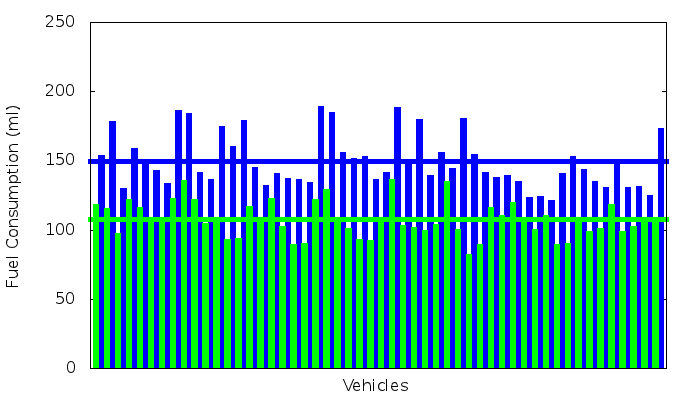
\includegraphics[width=0.5\textwidth]{images/tp0/fuelRoute.png}
\caption{Fuel graph}
\label{fig:TestResults:fuelRoute}
\end{figure}


%
\begin{figure}
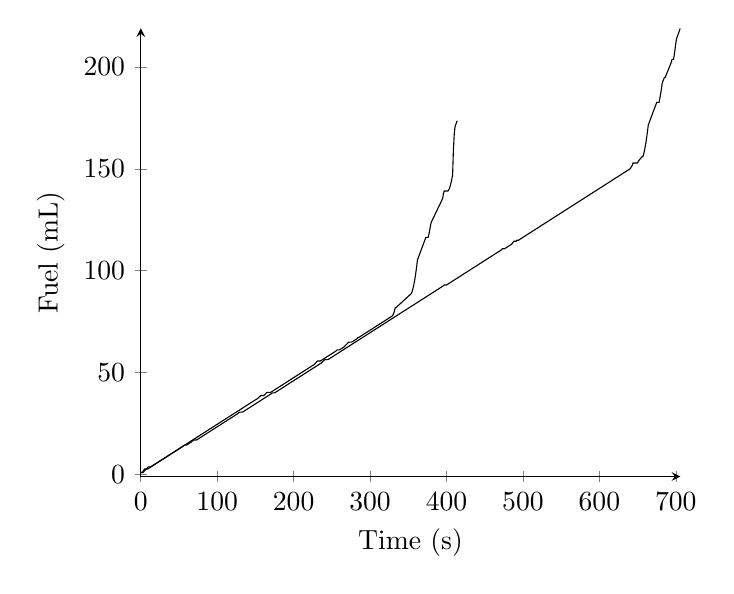
\begin{tikzpicture}
\begin{axis}[
legend style={anchor=west},
axis x line=bottom,
axis y line=left,
ymin=-1,
xlabel=Time (s),
ylabel=Fuel (mL),
]
\addplot[] coordinates {
(0, 1.00398986302)
(1, 1.00398986302)
(2, 1.00398986302)
(3, 1.00398986302)
(4, 1.39515894117)
(5, 1.78752409557)
(6, 2.18121563042)
(7, 2.57638382676)
(8, 2.97320299782)
(9, 3.37187659311)
(10, 3.77264368734)
(11, 3.77264368734)
(12, 3.77264368734)
(13, 3.77264368734)
(14, 4.0125292007)
(15, 4.25241471406)
(16, 4.49230022743)
(17, 4.73218574079)
(18, 4.97207125415)
(19, 5.21195676751)
(20, 5.45184228087)
(21, 5.69172779423)
(22, 5.93161330759)
(23, 6.17149882096)
(24, 6.41138433432)
(25, 6.65126984768)
(26, 6.89115536104)
(27, 7.1310408744)
(28, 7.37092638776)
(29, 7.61081190112)
(30, 7.85069741449)
(31, 8.09058292785)
(32, 8.33046844121)
(33, 8.57035395457)
(34, 8.81023946793)
(35, 9.05012498129)
(36, 9.29001049465)
(37, 9.52989600802)
(38, 9.76978152138)
(39, 10.0096670347)
(40, 10.2495525481)
(41, 10.4894380615)
(42, 10.7293235748)
(43, 10.9692090882)
(44, 11.2090946015)
(45, 11.4489801149)
(46, 11.6888656283)
(47, 11.9287511416)
(48, 12.168636655)
(49, 12.4085221684)
(50, 12.6484076817)
(51, 12.8882931951)
(52, 13.1281787084)
(53, 13.3680642218)
(54, 13.6079497352)
(55, 13.8478352485)
(56, 14.0877207619)
(57, 14.3276062752)
(58, 14.5674917886)
(59, 14.807377302)
(60, 15.0472628153)
(61, 15.2871483287)
(62, 15.5270338421)
(63, 15.7669193554)
(64, 16.0068048688)
(65, 16.2466903821)
(66, 16.4865758955)
(67, 16.7264614089)
(68, 16.9663469222)
(69, 17.2062324356)
(70, 17.4461179489)
(71, 17.6860034623)
(72, 17.9258889757)
(73, 18.165774489)
(74, 18.4056600024)
(75, 18.6455455158)
(76, 18.8854310291)
(77, 19.1253165425)
(78, 19.3652020558)
(79, 19.6050875692)
(80, 19.8449730826)
(81, 20.0848585959)
(82, 20.3247441093)
(83, 20.5646296226)
(84, 20.804515136)
(85, 21.0444006494)
(86, 21.2842861627)
(87, 21.5241716761)
(88, 21.7640571895)
(89, 22.0039427028)
(90, 22.2438282162)
(91, 22.4837137295)
(92, 22.7235992429)
(93, 22.9634847563)
(94, 23.2033702696)
(95, 23.443255783)
(96, 23.6831412963)
(97, 23.9230268097)
(98, 24.1629123231)
(99, 24.4027978364)
(100, 24.6426833498)
(101, 24.8825688631)
(102, 25.1224543765)
(103, 25.3623398899)
(104, 25.6022254032)
(105, 25.8421109166)
(106, 26.08199643)
(107, 26.3218819433)
(108, 26.5617674567)
(109, 26.80165297)
(110, 27.0415384834)
(111, 27.2814239968)
(112, 27.5213095101)
(113, 27.7611950235)
(114, 28.0010805368)
(115, 28.2409660502)
(116, 28.4808515636)
(117, 28.7207370769)
(118, 28.9606225903)
(119, 29.2005081037)
(120, 29.440393617)
(121, 29.6802791304)
(122, 29.9201646437)
(123, 30.1600501571)
(124, 30.3999356705)
(125, 30.6398211838)
(126, 30.8797066972)
(127, 31.1195922105)
(128, 31.3594777239)
(129, 31.5993632373)
(130, 31.8392487506)
(131, 32.079134264)
(132, 32.3190197774)
(133, 32.5589052907)
(134, 32.7987908041)
(135, 33.0386763174)
(136, 33.2785618308)
(137, 33.5184473442)
(138, 33.7583328575)
(139, 33.9982183709)
(140, 34.2381038842)
(141, 34.4779893976)
(142, 34.717874911)
(143, 34.9577604243)
(144, 35.1976459377)
(145, 35.4375314511)
(146, 35.6774169644)
(147, 35.9173024778)
(148, 36.1571879911)
(149, 36.3970735045)
(150, 36.6369590179)
(151, 36.8768445312)
(152, 37.1167300446)
(153, 37.3566155579)
(154, 37.6754102861)
(155, 38.0214797797)
(156, 38.3982514099)
(157, 38.7773300426)
(158, 38.7773300426)
(159, 38.7773300426)
(160, 38.7773300426)
(161, 38.7773300426)
(162, 39.1131872874)
(163, 39.4863461167)
(164, 39.9107983425)
(165, 40.3354002584)
(166, 40.3354002584)
(167, 40.3354002584)
(168, 40.3354002584)
(169, 40.3354002584)
(170, 40.3354002584)
(171, 40.5752857718)
(172, 40.8151712852)
(173, 41.0550567985)
(174, 41.2949423119)
(175, 41.5348278252)
(176, 41.7747133386)
(177, 42.014598852)
(178, 42.2544843653)
(179, 42.4943698787)
(180, 42.7342553921)
(181, 42.9741409054)
(182, 43.2140264188)
(183, 43.4539119321)
(184, 43.6937974455)
(185, 43.9336829589)
(186, 44.1735684722)
(187, 44.4134539856)
(188, 44.6533394989)
(189, 44.8932250123)
(190, 45.1331105257)
(191, 45.372996039)
(192, 45.6128815524)
(193, 45.8527670657)
(194, 46.0926525791)
(195, 46.3325380925)
(196, 46.5724236058)
(197, 46.8123091192)
(198, 47.0521946326)
(199, 47.2920801459)
(200, 47.5319656593)
(201, 47.7718511726)
(202, 48.011736686)
(203, 48.2516221994)
(204, 48.4915077127)
(205, 48.7313932261)
(206, 48.9712787394)
(207, 49.2111642528)
(208, 49.4510497662)
(209, 49.6909352795)
(210, 49.9308207929)
(211, 50.1707063063)
(212, 50.4105918196)
(213, 50.650477333)
(214, 50.8903628463)
(215, 51.1302483597)
(216, 51.3701338731)
(217, 51.6100193864)
(218, 51.8499048998)
(219, 52.0897904131)
(220, 52.3296759265)
(221, 52.5695614399)
(222, 52.8094469532)
(223, 53.0493324666)
(224, 53.28921798)
(225, 53.5291034933)
(226, 53.7689890067)
(227, 54.00887452)
(228, 54.3739405963)
(229, 54.7907220772)
(230, 55.2962563616)
(231, 55.7224306275)
(232, 55.7224306275)
(233, 55.7224306275)
(234, 55.7224306275)
(235, 55.7224306275)
(236, 55.9623161409)
(237, 56.2022016542)
(238, 56.4420871676)
(239, 56.681972681)
(240, 56.9218581943)
(241, 57.1617437077)
(242, 57.401629221)
(243, 57.6415147344)
(244, 57.8814002478)
(245, 58.1212857611)
(246, 58.3611712745)
(247, 58.6010567878)
(248, 58.8409423012)
(249, 59.0808278146)
(250, 59.3207133279)
(251, 59.5605988413)
(252, 59.8004843547)
(253, 60.040369868)
(254, 60.2802553814)
(255, 60.5201408947)
(256, 60.7600264081)
(257, 61.1665134408)
(258, 61.1665134408)
(259, 61.1665134408)
(260, 61.1665134408)
(261, 61.4063989542)
(262, 61.6462844675)
(263, 61.8861699809)
(264, 62.1260554942)
(265, 62.3659410076)
(266, 62.605826521)
(267, 63.0166362229)
(268, 63.4078408696)
(269, 63.7760199084)
(270, 64.1385374737)
(271, 64.6014662819)
(272, 64.993525959)
(273, 64.993525959)
(274, 64.993525959)
(275, 64.993525959)
(276, 64.993525959)
(277, 65.2334114723)
(278, 65.4732969857)
(279, 65.7131824991)
(280, 65.9530680124)
(281, 66.1929535258)
(282, 66.4328390391)
(283, 66.6727245525)
(284, 67.2382231329)
(285, 67.2382231329)
(286, 67.4781086463)
(287, 67.7179941596)
(288, 67.957879673)
(289, 68.1977651864)
(290, 68.4376506997)
(291, 68.6775362131)
(292, 68.9174217264)
(293, 69.1573072398)
(294, 69.3971927532)
(295, 69.6370782665)
(296, 69.8769637799)
(297, 70.1168492933)
(298, 70.3567348066)
(299, 70.59662032)
(300, 70.8365058333)
(301, 71.0763913467)
(302, 71.3162768601)
(303, 71.5561623734)
(304, 71.7960478868)
(305, 72.0359334001)
(306, 72.2758189135)
(307, 72.5157044269)
(308, 72.7555899402)
(309, 72.9954754536)
(310, 73.235360967)
(311, 73.4752464803)
(312, 73.7151319937)
(313, 73.955017507)
(314, 74.1949030204)
(315, 74.4347885338)
(316, 74.6746740471)
(317, 74.9145595605)
(318, 75.1544450738)
(319, 75.3943305872)
(320, 75.6342161006)
(321, 75.8741016139)
(322, 76.1139871273)
(323, 76.3538726407)
(324, 76.593758154)
(325, 76.8336436674)
(326, 77.0735291807)
(327, 77.3134146941)
(328, 77.5533002075)
(329, 77.7931857208)
(330, 78.3586843012)
(331, 79.2433215389)
(332, 80.4430316923)
(333, 81.9561576881)
(334, 81.9561576881)
(335, 82.2983700713)
(336, 82.6405956491)
(337, 82.9828364747)
(338, 83.32509505)
(339, 83.6673744553)
(340, 84.0096785264)
(341, 84.3520121024)
(342, 84.6943757251)
(343, 85.0368957377)
(344, 85.3793951584)
(345, 85.7219634925)
(346, 86.0646208839)
(347, 86.4073962379)
(348, 86.7503326381)
(349, 87.0934974511)
(350, 87.4370028071)
(351, 87.781052092)
(352, 88.1260643712)
(353, 88.4731095639)
(354, 88.8265351434)
(355, 89.79628684)
(356, 91.0804284578)
(357, 92.6779513154)
(358, 94.590255399)
(359, 96.8211493635)
(360, 99.3768505317)
(361, 102.265984895)
(362, 105.340332541)
(363, 106.344322404)
(364, 107.348312267)
(365, 108.35230213)
(366, 109.356291993)
(367, 110.360281856)
(368, 111.364271719)
(369, 112.368261582)
(370, 113.372251445)
(371, 114.376241308)
(372, 115.380231171)
(373, 116.384221035)
(374, 116.384221035)
(375, 116.384221035)
(376, 116.384221035)
(377, 117.983616297)
(378, 119.897808375)
(379, 122.130620299)
(380, 123.758840511)
(381, 124.537038064)
(382, 125.315398648)
(383, 126.093958488)
(384, 126.872764897)
(385, 127.651880729)
(386, 128.43139109)
(387, 129.21141375)
(388, 130.00345177)
(389, 130.783044079)
(390, 131.562774005)
(391, 132.342703216)
(392, 133.122933708)
(393, 133.903645094)
(394, 134.685180356)
(395, 135.46801956)
(396, 137.907749419)
(397, 139.114437489)
(398, 139.114437489)
(399, 139.114437489)
(400, 139.114437489)
(401, 139.114437489)
(402, 139.114437489)
(403, 139.679936069)
(404, 140.564573307)
(405, 141.76428346)
(406, 143.277409456)
(407, 145.104702889)
(408, 147.249324022)
(409, 159.067779967)
(410, 166.417953869)
(411, 170.270438334)
(412, 171.619915219)
(413, 172.623905082)
(414, 173.627894945)
};
\addplot[] coordinates {
(0, 1.00398986302)
(1, 1.00398986302)
(2, 1.00398986302)
(3, 1.56220432482)
(4, 2.12998612821)
(5, 2.71016271768)
(6, 2.71016271768)
(7, 2.71016271768)
(8, 2.71016271768)
(9, 2.71016271768)
(10, 2.95004823104)
(11, 3.18993374441)
(12, 3.42981925777)
(13, 3.66970477113)
(14, 3.90959028449)
(15, 4.14947579785)
(16, 4.38936131121)
(17, 4.62924682458)
(18, 4.86913233794)
(19, 5.1090178513)
(20, 5.34890336466)
(21, 5.58878887802)
(22, 5.82867439138)
(23, 6.06855990474)
(24, 6.30844541811)
(25, 6.54833093147)
(26, 6.78821644483)
(27, 7.02810195819)
(28, 7.26798747155)
(29, 7.50787298491)
(30, 7.74775849827)
(31, 7.98764401164)
(32, 8.227529525)
(33, 8.46741503836)
(34, 8.70730055172)
(35, 8.94718606508)
(36, 9.18707157844)
(37, 9.4269570918)
(38, 9.66684260517)
(39, 9.90672811853)
(40, 10.1466136319)
(41, 10.3864991453)
(42, 10.6263846586)
(43, 10.866270172)
(44, 11.1061556853)
(45, 11.3460411987)
(46, 11.5859267121)
(47, 11.8258122254)
(48, 12.0656977388)
(49, 12.3055832521)
(50, 12.5454687655)
(51, 12.7853542789)
(52, 13.0252397922)
(53, 13.2651253056)
(54, 13.5050108189)
(55, 13.8135613533)
(56, 14.1412035385)
(57, 14.4479651751)
(58, 14.4479651751)
(59, 14.4479651751)
(60, 14.4479651751)
(61, 14.6878506885)
(62, 14.9277362018)
(63, 15.1676217152)
(64, 15.4075072286)
(65, 15.6473927419)
(66, 15.8872782553)
(67, 16.2136550252)
(68, 16.5665482079)
(69, 16.938787415)
(70, 16.938787415)
(71, 16.938787415)
(72, 16.938787415)
(73, 16.938787415)
(74, 17.1786729284)
(75, 17.4185584418)
(76, 17.6584439551)
(77, 17.8983294685)
(78, 18.1382149819)
(79, 18.3781004952)
(80, 18.6179860086)
(81, 18.8578715219)
(82, 19.0977570353)
(83, 19.3376425487)
(84, 19.577528062)
(85, 19.8174135754)
(86, 20.0572990887)
(87, 20.2971846021)
(88, 20.5370701155)
(89, 20.7769556288)
(90, 21.0168411422)
(91, 21.2567266556)
(92, 21.4966121689)
(93, 21.7364976823)
(94, 21.9763831956)
(95, 22.216268709)
(96, 22.4561542224)
(97, 22.6960397357)
(98, 22.9359252491)
(99, 23.1758107624)
(100, 23.4156962758)
(101, 23.6555817892)
(102, 23.8954673025)
(103, 24.1353528159)
(104, 24.3752383293)
(105, 24.6151238426)
(106, 24.855009356)
(107, 25.0948948693)
(108, 25.3347803827)
(109, 25.5746658961)
(110, 25.8145514094)
(111, 26.0544369228)
(112, 26.2943224361)
(113, 26.5342079495)
(114, 26.7740934629)
(115, 27.0139789762)
(116, 27.2538644896)
(117, 27.493750003)
(118, 27.7336355163)
(119, 27.9735210297)
(120, 28.213406543)
(121, 28.4532920564)
(122, 28.6931775698)
(123, 28.9330630831)
(124, 29.1729485965)
(125, 29.4128341098)
(126, 29.6527196232)
(127, 29.8926051366)
(128, 30.2295784714)
(129, 30.5816510348)
(130, 30.5816510348)
(131, 30.5816510348)
(132, 30.5816510348)
(133, 30.5816510348)
(134, 30.8215365482)
(135, 31.0614220615)
(136, 31.3013075749)
(137, 31.5411930882)
(138, 31.7810786016)
(139, 32.020964115)
(140, 32.2608496283)
(141, 32.5007351417)
(142, 32.740620655)
(143, 32.9805061684)
(144, 33.2203916818)
(145, 33.4602771951)
(146, 33.7001627085)
(147, 33.9400482219)
(148, 34.1799337352)
(149, 34.4198192486)
(150, 34.6597047619)
(151, 34.8995902753)
(152, 35.1394757887)
(153, 35.379361302)
(154, 35.6192468154)
(155, 35.8591323287)
(156, 36.0990178421)
(157, 36.3389033555)
(158, 36.5787888688)
(159, 36.8186743822)
(160, 37.0585598956)
(161, 37.2984454089)
(162, 37.5383309223)
(163, 37.7782164356)
(164, 38.018101949)
(165, 38.2579874624)
(166, 38.4978729757)
(167, 38.7377584891)
(168, 38.9776440024)
(169, 39.2175295158)
(170, 39.4574150292)
(171, 39.6973005425)
(172, 40.0462181687)
(173, 40.0462181687)
(174, 40.0462181687)
(175, 40.0462181687)
(176, 40.286103682)
(177, 40.5259891954)
(178, 40.7658747088)
(179, 41.0057602221)
(180, 41.2456457355)
(181, 41.4855312488)
(182, 41.7254167622)
(183, 41.9653022756)
(184, 42.2051877889)
(185, 42.4450733023)
(186, 42.6849588156)
(187, 42.924844329)
(188, 43.1647298424)
(189, 43.4046153557)
(190, 43.6445008691)
(191, 43.8843863825)
(192, 44.1242718958)
(193, 44.3641574092)
(194, 44.6040429225)
(195, 44.8439284359)
(196, 45.0838139493)
(197, 45.3236994626)
(198, 45.563584976)
(199, 45.8034704893)
(200, 46.0433560027)
(201, 46.2832415161)
(202, 46.5231270294)
(203, 46.7630125428)
(204, 47.0028980562)
(205, 47.2427835695)
(206, 47.4826690829)
(207, 47.7225545962)
(208, 47.9624401096)
(209, 48.202325623)
(210, 48.4422111363)
(211, 48.6820966497)
(212, 48.921982163)
(213, 49.1618676764)
(214, 49.4017531898)
(215, 49.6416387031)
(216, 49.8815242165)
(217, 50.1214097299)
(218, 50.3612952432)
(219, 50.6011807566)
(220, 50.8410662699)
(221, 51.0809517833)
(222, 51.3208372967)
(223, 51.56072281)
(224, 51.8006083234)
(225, 52.0404938367)
(226, 52.2803793501)
(227, 52.5202648635)
(228, 52.7601503768)
(229, 53.0000358902)
(230, 53.2399214036)
(231, 53.4798069169)
(232, 53.7196924303)
(233, 53.9595779436)
(234, 54.199463457)
(235, 54.4393489704)
(236, 54.6792344837)
(237, 55.0280182903)
(238, 55.420201219)
(239, 55.7482252469)
(240, 56.0761294264)
(241, 56.4051411833)
(242, 56.4051411833)
(243, 56.4051411833)
(244, 56.4051411833)
(245, 56.4051411833)
(246, 56.6450266966)
(247, 56.88491221)
(248, 57.1247977234)
(249, 57.3646832367)
(250, 57.6045687501)
(251, 57.8444542634)
(252, 58.0843397768)
(253, 58.3242252902)
(254, 58.5641108035)
(255, 58.8039963169)
(256, 59.0438818302)
(257, 59.2837673436)
(258, 59.523652857)
(259, 59.7635383703)
(260, 60.0034238837)
(261, 60.243309397)
(262, 60.4831949104)
(263, 60.7230804238)
(264, 60.9629659371)
(265, 61.2028514505)
(266, 61.4427369639)
(267, 61.6826224772)
(268, 61.9225079906)
(269, 62.1623935039)
(270, 62.4022790173)
(271, 62.6421645307)
(272, 62.882050044)
(273, 63.1219355574)
(274, 63.3618210707)
(275, 63.6017065841)
(276, 63.8415920975)
(277, 64.0814776108)
(278, 64.3213631242)
(279, 64.5612486376)
(280, 64.8011341509)
(281, 65.0410196643)
(282, 65.2809051776)
(283, 65.520790691)
(284, 65.7606762044)
(285, 66.0005617177)
(286, 66.2404472311)
(287, 66.4803327444)
(288, 66.7202182578)
(289, 66.9601037712)
(290, 67.1999892845)
(291, 67.4398747979)
(292, 67.6797603113)
(293, 67.9196458246)
(294, 68.159531338)
(295, 68.3994168513)
(296, 68.6393023647)
(297, 68.8791878781)
(298, 69.1190733914)
(299, 69.3589589048)
(300, 69.5988444181)
(301, 69.8387299315)
(302, 70.0786154449)
(303, 70.3185009582)
(304, 70.5583864716)
(305, 70.798271985)
(306, 71.0381574983)
(307, 71.2780430117)
(308, 71.517928525)
(309, 71.7578140384)
(310, 71.9976995518)
(311, 72.2375850651)
(312, 72.4774705785)
(313, 72.7173560918)
(314, 72.9572416052)
(315, 73.1971271186)
(316, 73.4370126319)
(317, 73.6768981453)
(318, 73.9167836587)
(319, 74.156669172)
(320, 74.3965546854)
(321, 74.6364401987)
(322, 74.8763257121)
(323, 75.1162112255)
(324, 75.3560967388)
(325, 75.5959822522)
(326, 75.8358677655)
(327, 76.0757532789)
(328, 76.3156387923)
(329, 76.5555243056)
(330, 76.795409819)
(331, 77.0352953324)
(332, 77.2751808457)
(333, 77.5150663591)
(334, 77.7549518724)
(335, 77.9948373858)
(336, 78.2347228992)
(337, 78.4746084125)
(338, 78.7144939259)
(339, 78.9543794392)
(340, 79.1942649526)
(341, 79.434150466)
(342, 79.6740359793)
(343, 79.9139214927)
(344, 80.1538070061)
(345, 80.3936925194)
(346, 80.6335780328)
(347, 80.8734635461)
(348, 81.1133490595)
(349, 81.3532345729)
(350, 81.5931200862)
(351, 81.8330055996)
(352, 82.0728911129)
(353, 82.3127766263)
(354, 82.5526621397)
(355, 82.792547653)
(356, 83.0324331664)
(357, 83.2723186798)
(358, 83.5122041931)
(359, 83.7520897065)
(360, 83.9919752198)
(361, 84.2318607332)
(362, 84.4717462466)
(363, 84.7116317599)
(364, 84.9515172733)
(365, 85.1914027866)
(366, 85.4312883)
(367, 85.6711738134)
(368, 85.9110593267)
(369, 86.1509448401)
(370, 86.3908303534)
(371, 86.6307158668)
(372, 86.8706013802)
(373, 87.1104868935)
(374, 87.3503724069)
(375, 87.5902579203)
(376, 87.8301434336)
(377, 88.070028947)
(378, 88.3099144603)
(379, 88.5497999737)
(380, 88.7896854871)
(381, 89.0295710004)
(382, 89.2694565138)
(383, 89.5093420271)
(384, 89.7492275405)
(385, 89.9891130539)
(386, 90.2289985672)
(387, 90.4688840806)
(388, 90.708769594)
(389, 90.9486551073)
(390, 91.1885406207)
(391, 91.428426134)
(392, 91.6683116474)
(393, 91.9081971608)
(394, 92.1480826741)
(395, 92.3879681875)
(396, 92.6278537008)
(397, 93.0127159839)
(398, 93.0127159839)
(399, 93.0127159839)
(400, 93.0127159839)
(401, 93.2526014972)
(402, 93.4924870106)
(403, 93.732372524)
(404, 93.9722580373)
(405, 94.2121435507)
(406, 94.452029064)
(407, 94.6919145774)
(408, 94.9318000908)
(409, 95.1716856041)
(410, 95.4115711175)
(411, 95.6514566308)
(412, 95.8913421442)
(413, 96.1312276576)
(414, 96.3711131709)
(415, 96.6109986843)
(416, 96.8508841977)
(417, 97.090769711)
(418, 97.3306552244)
(419, 97.5705407377)
(420, 97.8104262511)
(421, 98.0503117645)
(422, 98.2901972778)
(423, 98.5300827912)
(424, 98.7699683045)
(425, 99.0098538179)
(426, 99.2497393313)
(427, 99.4896248446)
(428, 99.729510358)
(429, 99.9693958714)
(430, 100.209281385)
(431, 100.449166898)
(432, 100.689052411)
(433, 100.928937925)
(434, 101.168823438)
(435, 101.408708952)
(436, 101.648594465)
(437, 101.888479978)
(438, 102.128365492)
(439, 102.368251005)
(440, 102.608136518)
(441, 102.848022032)
(442, 103.087907545)
(443, 103.327793058)
(444, 103.567678572)
(445, 103.807564085)
(446, 104.047449598)
(447, 104.287335112)
(448, 104.527220625)
(449, 104.767106139)
(450, 105.006991652)
(451, 105.246877165)
(452, 105.486762679)
(453, 105.726648192)
(454, 105.966533705)
(455, 106.206419219)
(456, 106.446304732)
(457, 106.686190245)
(458, 106.926075759)
(459, 107.165961272)
(460, 107.405846786)
(461, 107.645732299)
(462, 107.885617812)
(463, 108.125503326)
(464, 108.365388839)
(465, 108.605274352)
(466, 108.845159866)
(467, 109.085045379)
(468, 109.324930892)
(469, 109.564816406)
(470, 109.804701919)
(471, 110.044587433)
(472, 110.428992117)
(473, 110.805973467)
(474, 110.805973467)
(475, 110.805973467)
(476, 110.805973467)
(477, 111.04585898)
(478, 111.285744493)
(479, 111.525630007)
(480, 111.76551552)
(481, 112.005401033)
(482, 112.245286547)
(483, 112.48517206)
(484, 112.725057574)
(485, 112.964943087)
(486, 113.376162188)
(487, 113.873501298)
(488, 114.481196488)
(489, 114.481196488)
(490, 114.481196488)
(491, 114.481196488)
(492, 114.95345684)
(493, 114.95345684)
(494, 114.95345684)
(495, 115.193342353)
(496, 115.433227866)
(497, 115.67311338)
(498, 115.912998893)
(499, 116.152884406)
(500, 116.39276992)
(501, 116.632655433)
(502, 116.872540946)
(503, 117.11242646)
(504, 117.352311973)
(505, 117.592197487)
(506, 117.832083)
(507, 118.071968513)
(508, 118.311854027)
(509, 118.55173954)
(510, 118.791625053)
(511, 119.031510567)
(512, 119.27139608)
(513, 119.511281593)
(514, 119.751167107)
(515, 119.99105262)
(516, 120.230938134)
(517, 120.470823647)
(518, 120.71070916)
(519, 120.950594674)
(520, 121.190480187)
(521, 121.4303657)
(522, 121.670251214)
(523, 121.910136727)
(524, 122.15002224)
(525, 122.389907754)
(526, 122.629793267)
(527, 122.869678781)
(528, 123.109564294)
(529, 123.349449807)
(530, 123.589335321)
(531, 123.829220834)
(532, 124.069106347)
(533, 124.308991861)
(534, 124.548877374)
(535, 124.788762887)
(536, 125.028648401)
(537, 125.268533914)
(538, 125.508419427)
(539, 125.748304941)
(540, 125.988190454)
(541, 126.228075968)
(542, 126.467961481)
(543, 126.707846994)
(544, 126.947732508)
(545, 127.187618021)
(546, 127.427503534)
(547, 127.667389048)
(548, 127.907274561)
(549, 128.147160074)
(550, 128.387045588)
(551, 128.626931101)
(552, 128.866816615)
(553, 129.106702128)
(554, 129.346587641)
(555, 129.586473155)
(556, 129.826358668)
(557, 130.066244181)
(558, 130.306129695)
(559, 130.546015208)
(560, 130.785900721)
(561, 131.025786235)
(562, 131.265671748)
(563, 131.505557262)
(564, 131.745442775)
(565, 131.985328288)
(566, 132.225213802)
(567, 132.465099315)
(568, 132.704984828)
(569, 132.944870342)
(570, 133.184755855)
(571, 133.424641368)
(572, 133.664526882)
(573, 133.904412395)
(574, 134.144297908)
(575, 134.384183422)
(576, 134.624068935)
(577, 134.863954449)
(578, 135.103839962)
(579, 135.343725475)
(580, 135.583610989)
(581, 135.823496502)
(582, 136.063382015)
(583, 136.303267529)
(584, 136.543153042)
(585, 136.783038555)
(586, 137.022924069)
(587, 137.262809582)
(588, 137.502695096)
(589, 137.742580609)
(590, 137.982466122)
(591, 138.222351636)
(592, 138.462237149)
(593, 138.702122662)
(594, 138.942008176)
(595, 139.181893689)
(596, 139.421779202)
(597, 139.661664716)
(598, 139.901550229)
(599, 140.141435743)
(600, 140.381321256)
(601, 140.621206769)
(602, 140.861092283)
(603, 141.100977796)
(604, 141.340863309)
(605, 141.580748823)
(606, 141.820634336)
(607, 142.060519849)
(608, 142.300405363)
(609, 142.540290876)
(610, 142.78017639)
(611, 143.020061903)
(612, 143.259947416)
(613, 143.49983293)
(614, 143.739718443)
(615, 143.979603956)
(616, 144.21948947)
(617, 144.459374983)
(618, 144.699260496)
(619, 144.93914601)
(620, 145.179031523)
(621, 145.418917036)
(622, 145.65880255)
(623, 145.898688063)
(624, 146.138573577)
(625, 146.37845909)
(626, 146.618344603)
(627, 146.858230117)
(628, 147.09811563)
(629, 147.338001143)
(630, 147.577886657)
(631, 147.81777217)
(632, 148.057657683)
(633, 148.297543197)
(634, 148.53742871)
(635, 148.777314224)
(636, 149.017199737)
(637, 149.25708525)
(638, 149.496970764)
(639, 149.736856277)
(640, 149.97674179)
(641, 150.472180293)
(642, 151.154140033)
(643, 151.685004764)
(644, 152.894087411)
(645, 152.894087411)
(646, 152.894087411)
(647, 152.894087411)
(648, 152.894087411)
(649, 152.894087411)
(650, 152.894087411)
(651, 153.798361732)
(652, 154.249845037)
(653, 154.702265904)
(654, 155.155101242)
(655, 155.609558032)
(656, 156.068036742)
(657, 156.068036742)
(658, 157.370761926)
(659, 158.986884183)
(660, 160.917946299)
(661, 163.16789973)
(662, 165.743104598)
(663, 168.652329696)
(664, 171.552107284)
(665, 172.556097147)
(666, 173.56008701)
(667, 174.564076873)
(668, 175.568066736)
(669, 176.572056599)
(670, 177.576046462)
(671, 178.580036325)
(672, 179.584026188)
(673, 180.588016051)
(674, 181.592005914)
(675, 182.595995777)
(676, 182.595995777)
(677, 182.595995777)
(678, 182.595995777)
(679, 184.358877575)
(680, 186.438245051)
(681, 188.83917467)
(682, 191.569151567)
(683, 192.949218616)
(684, 193.841802856)
(685, 194.847525197)
(686, 194.847525197)
(687, 195.765539893)
(688, 196.685040856)
(689, 197.605908091)
(690, 198.523001034)
(691, 199.441058808)
(692, 200.360673408)
(693, 201.282992658)
(694, 202.210512329)
(695, 203.757183275)
(696, 203.757183275)
(697, 203.757183275)
(698, 206.082005509)
(699, 208.733900597)
(700, 211.722196625)
(701, 213.998175848)
(702, 215.002165711)
(703, 216.006155574)
(704, 217.010145437)
(705, 218.0141353)
(706, 219.018125163)
};

\end{axis}
\end{tikzpicture}
\label{tik:fuel:100:51}
\caption{100 percent diving with GSC on route $51$}
\end{figure}

%
\begin{figure}
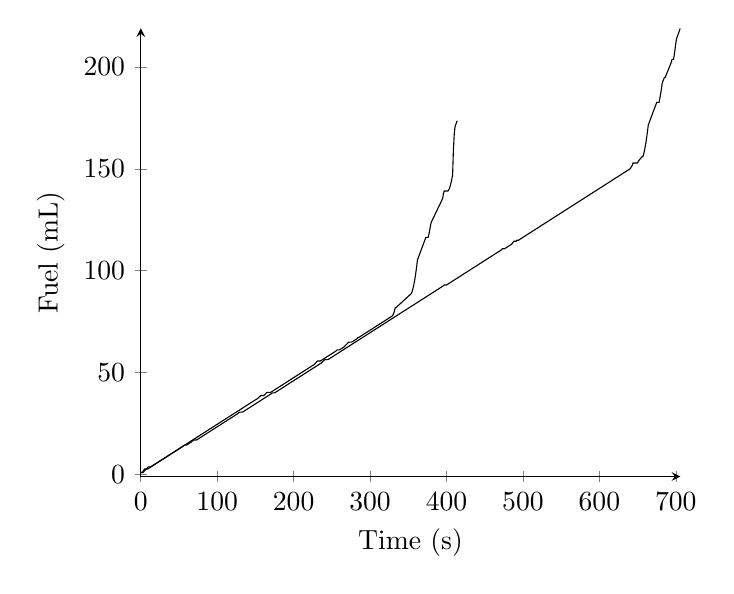
\begin{tikzpicture}
\begin{axis}[
legend style={anchor=west},
axis x line=bottom,
axis y line=left,
ymin=-1,
xlabel=Time (s),
ylabel=Fuel (mL),
]
\addplot[] coordinates {
(0, 1.00398986302)
(1, 1.00398986302)
(2, 1.00398986302)
(3, 1.00398986302)
(4, 1.39515894117)
(5, 1.78752409557)
(6, 2.18121563042)
(7, 2.57638382676)
(8, 2.97320299782)
(9, 3.37187659311)
(10, 3.77264368734)
(11, 3.77264368734)
(12, 3.77264368734)
(13, 3.77264368734)
(14, 4.0125292007)
(15, 4.25241471406)
(16, 4.49230022743)
(17, 4.73218574079)
(18, 4.97207125415)
(19, 5.21195676751)
(20, 5.45184228087)
(21, 5.69172779423)
(22, 5.93161330759)
(23, 6.17149882096)
(24, 6.41138433432)
(25, 6.65126984768)
(26, 6.89115536104)
(27, 7.1310408744)
(28, 7.37092638776)
(29, 7.61081190112)
(30, 7.85069741449)
(31, 8.09058292785)
(32, 8.33046844121)
(33, 8.57035395457)
(34, 8.81023946793)
(35, 9.05012498129)
(36, 9.29001049465)
(37, 9.52989600802)
(38, 9.76978152138)
(39, 10.0096670347)
(40, 10.2495525481)
(41, 10.4894380615)
(42, 10.7293235748)
(43, 10.9692090882)
(44, 11.2090946015)
(45, 11.4489801149)
(46, 11.6888656283)
(47, 11.9287511416)
(48, 12.168636655)
(49, 12.4085221684)
(50, 12.6484076817)
(51, 12.8882931951)
(52, 13.1281787084)
(53, 13.3680642218)
(54, 13.6079497352)
(55, 13.8478352485)
(56, 14.0877207619)
(57, 14.3276062752)
(58, 14.5674917886)
(59, 14.807377302)
(60, 15.0472628153)
(61, 15.2871483287)
(62, 15.5270338421)
(63, 15.7669193554)
(64, 16.0068048688)
(65, 16.2466903821)
(66, 16.4865758955)
(67, 16.7264614089)
(68, 16.9663469222)
(69, 17.2062324356)
(70, 17.4461179489)
(71, 17.6860034623)
(72, 17.9258889757)
(73, 18.165774489)
(74, 18.4056600024)
(75, 18.6455455158)
(76, 18.8854310291)
(77, 19.1253165425)
(78, 19.3652020558)
(79, 19.6050875692)
(80, 19.8449730826)
(81, 20.0848585959)
(82, 20.3247441093)
(83, 20.5646296226)
(84, 20.804515136)
(85, 21.0444006494)
(86, 21.2842861627)
(87, 21.5241716761)
(88, 21.7640571895)
(89, 22.0039427028)
(90, 22.2438282162)
(91, 22.4837137295)
(92, 22.7235992429)
(93, 22.9634847563)
(94, 23.2033702696)
(95, 23.443255783)
(96, 23.6831412963)
(97, 23.9230268097)
(98, 24.1629123231)
(99, 24.4027978364)
(100, 24.6426833498)
(101, 24.8825688631)
(102, 25.1224543765)
(103, 25.3623398899)
(104, 25.6022254032)
(105, 25.8421109166)
(106, 26.08199643)
(107, 26.3218819433)
(108, 26.5617674567)
(109, 26.80165297)
(110, 27.0415384834)
(111, 27.2814239968)
(112, 27.5213095101)
(113, 27.7611950235)
(114, 28.0010805368)
(115, 28.2409660502)
(116, 28.4808515636)
(117, 28.7207370769)
(118, 28.9606225903)
(119, 29.2005081037)
(120, 29.440393617)
(121, 29.6802791304)
(122, 29.9201646437)
(123, 30.1600501571)
(124, 30.3999356705)
(125, 30.6398211838)
(126, 30.8797066972)
(127, 31.1195922105)
(128, 31.3594777239)
(129, 31.5993632373)
(130, 31.8392487506)
(131, 32.079134264)
(132, 32.3190197774)
(133, 32.5589052907)
(134, 32.7987908041)
(135, 33.0386763174)
(136, 33.2785618308)
(137, 33.5184473442)
(138, 33.7583328575)
(139, 33.9982183709)
(140, 34.2381038842)
(141, 34.4779893976)
(142, 34.717874911)
(143, 34.9577604243)
(144, 35.1976459377)
(145, 35.4375314511)
(146, 35.6774169644)
(147, 35.9173024778)
(148, 36.1571879911)
(149, 36.3970735045)
(150, 36.6369590179)
(151, 36.8768445312)
(152, 37.1167300446)
(153, 37.3566155579)
(154, 37.6754102861)
(155, 38.0214797797)
(156, 38.3982514099)
(157, 38.7773300426)
(158, 38.7773300426)
(159, 38.7773300426)
(160, 38.7773300426)
(161, 38.7773300426)
(162, 39.1131872874)
(163, 39.4863461167)
(164, 39.9107983425)
(165, 40.3354002584)
(166, 40.3354002584)
(167, 40.3354002584)
(168, 40.3354002584)
(169, 40.3354002584)
(170, 40.3354002584)
(171, 40.5752857718)
(172, 40.8151712852)
(173, 41.0550567985)
(174, 41.2949423119)
(175, 41.5348278252)
(176, 41.7747133386)
(177, 42.014598852)
(178, 42.2544843653)
(179, 42.4943698787)
(180, 42.7342553921)
(181, 42.9741409054)
(182, 43.2140264188)
(183, 43.4539119321)
(184, 43.6937974455)
(185, 43.9336829589)
(186, 44.1735684722)
(187, 44.4134539856)
(188, 44.6533394989)
(189, 44.8932250123)
(190, 45.1331105257)
(191, 45.372996039)
(192, 45.6128815524)
(193, 45.8527670657)
(194, 46.0926525791)
(195, 46.3325380925)
(196, 46.5724236058)
(197, 46.8123091192)
(198, 47.0521946326)
(199, 47.2920801459)
(200, 47.5319656593)
(201, 47.7718511726)
(202, 48.011736686)
(203, 48.2516221994)
(204, 48.4915077127)
(205, 48.7313932261)
(206, 48.9712787394)
(207, 49.2111642528)
(208, 49.4510497662)
(209, 49.6909352795)
(210, 49.9308207929)
(211, 50.1707063063)
(212, 50.4105918196)
(213, 50.650477333)
(214, 50.8903628463)
(215, 51.1302483597)
(216, 51.3701338731)
(217, 51.6100193864)
(218, 51.8499048998)
(219, 52.0897904131)
(220, 52.3296759265)
(221, 52.5695614399)
(222, 52.8094469532)
(223, 53.0493324666)
(224, 53.28921798)
(225, 53.5291034933)
(226, 53.7689890067)
(227, 54.00887452)
(228, 54.3739405963)
(229, 54.7907220772)
(230, 55.2962563616)
(231, 55.7224306275)
(232, 55.7224306275)
(233, 55.7224306275)
(234, 55.7224306275)
(235, 55.7224306275)
(236, 55.9623161409)
(237, 56.2022016542)
(238, 56.4420871676)
(239, 56.681972681)
(240, 56.9218581943)
(241, 57.1617437077)
(242, 57.401629221)
(243, 57.6415147344)
(244, 57.8814002478)
(245, 58.1212857611)
(246, 58.3611712745)
(247, 58.6010567878)
(248, 58.8409423012)
(249, 59.0808278146)
(250, 59.3207133279)
(251, 59.5605988413)
(252, 59.8004843547)
(253, 60.040369868)
(254, 60.2802553814)
(255, 60.5201408947)
(256, 60.7600264081)
(257, 61.1665134408)
(258, 61.1665134408)
(259, 61.1665134408)
(260, 61.1665134408)
(261, 61.4063989542)
(262, 61.6462844675)
(263, 61.8861699809)
(264, 62.1260554942)
(265, 62.3659410076)
(266, 62.605826521)
(267, 63.0166362229)
(268, 63.4078408696)
(269, 63.7760199084)
(270, 64.1385374737)
(271, 64.6014662819)
(272, 64.993525959)
(273, 64.993525959)
(274, 64.993525959)
(275, 64.993525959)
(276, 64.993525959)
(277, 65.2334114723)
(278, 65.4732969857)
(279, 65.7131824991)
(280, 65.9530680124)
(281, 66.1929535258)
(282, 66.4328390391)
(283, 66.6727245525)
(284, 67.2382231329)
(285, 67.2382231329)
(286, 67.4781086463)
(287, 67.7179941596)
(288, 67.957879673)
(289, 68.1977651864)
(290, 68.4376506997)
(291, 68.6775362131)
(292, 68.9174217264)
(293, 69.1573072398)
(294, 69.3971927532)
(295, 69.6370782665)
(296, 69.8769637799)
(297, 70.1168492933)
(298, 70.3567348066)
(299, 70.59662032)
(300, 70.8365058333)
(301, 71.0763913467)
(302, 71.3162768601)
(303, 71.5561623734)
(304, 71.7960478868)
(305, 72.0359334001)
(306, 72.2758189135)
(307, 72.5157044269)
(308, 72.7555899402)
(309, 72.9954754536)
(310, 73.235360967)
(311, 73.4752464803)
(312, 73.7151319937)
(313, 73.955017507)
(314, 74.1949030204)
(315, 74.4347885338)
(316, 74.6746740471)
(317, 74.9145595605)
(318, 75.1544450738)
(319, 75.3943305872)
(320, 75.6342161006)
(321, 75.8741016139)
(322, 76.1139871273)
(323, 76.3538726407)
(324, 76.593758154)
(325, 76.8336436674)
(326, 77.0735291807)
(327, 77.3134146941)
(328, 77.5533002075)
(329, 77.7931857208)
(330, 78.3586843012)
(331, 79.2433215389)
(332, 80.4430316923)
(333, 81.9561576881)
(334, 81.9561576881)
(335, 82.2983700713)
(336, 82.6405956491)
(337, 82.9828364747)
(338, 83.32509505)
(339, 83.6673744553)
(340, 84.0096785264)
(341, 84.3520121024)
(342, 84.6943757251)
(343, 85.0368957377)
(344, 85.3793951584)
(345, 85.7219634925)
(346, 86.0646208839)
(347, 86.4073962379)
(348, 86.7503326381)
(349, 87.0934974511)
(350, 87.4370028071)
(351, 87.781052092)
(352, 88.1260643712)
(353, 88.4731095639)
(354, 88.8265351434)
(355, 89.79628684)
(356, 91.0804284578)
(357, 92.6779513154)
(358, 94.590255399)
(359, 96.8211493635)
(360, 99.3768505317)
(361, 102.265984895)
(362, 105.340332541)
(363, 106.344322404)
(364, 107.348312267)
(365, 108.35230213)
(366, 109.356291993)
(367, 110.360281856)
(368, 111.364271719)
(369, 112.368261582)
(370, 113.372251445)
(371, 114.376241308)
(372, 115.380231171)
(373, 116.384221035)
(374, 116.384221035)
(375, 116.384221035)
(376, 116.384221035)
(377, 117.983616297)
(378, 119.897808375)
(379, 122.130620299)
(380, 123.758840511)
(381, 124.537038064)
(382, 125.315398648)
(383, 126.093958488)
(384, 126.872764897)
(385, 127.651880729)
(386, 128.43139109)
(387, 129.21141375)
(388, 130.00345177)
(389, 130.783044079)
(390, 131.562774005)
(391, 132.342703216)
(392, 133.122933708)
(393, 133.903645094)
(394, 134.685180356)
(395, 135.46801956)
(396, 137.907749419)
(397, 139.114437489)
(398, 139.114437489)
(399, 139.114437489)
(400, 139.114437489)
(401, 139.114437489)
(402, 139.114437489)
(403, 139.679936069)
(404, 140.564573307)
(405, 141.76428346)
(406, 143.277409456)
(407, 145.104702889)
(408, 147.249324022)
(409, 159.067779967)
(410, 166.417953869)
(411, 170.270438334)
(412, 171.619915219)
(413, 172.623905082)
(414, 173.627894945)
};
\addplot[] coordinates {
(0, 1.00398986302)
(1, 1.00398986302)
(2, 1.00398986302)
(3, 1.56220432482)
(4, 2.12998612821)
(5, 2.71016271768)
(6, 2.71016271768)
(7, 2.71016271768)
(8, 2.71016271768)
(9, 2.71016271768)
(10, 2.95004823104)
(11, 3.18993374441)
(12, 3.42981925777)
(13, 3.66970477113)
(14, 3.90959028449)
(15, 4.14947579785)
(16, 4.38936131121)
(17, 4.62924682458)
(18, 4.86913233794)
(19, 5.1090178513)
(20, 5.34890336466)
(21, 5.58878887802)
(22, 5.82867439138)
(23, 6.06855990474)
(24, 6.30844541811)
(25, 6.54833093147)
(26, 6.78821644483)
(27, 7.02810195819)
(28, 7.26798747155)
(29, 7.50787298491)
(30, 7.74775849827)
(31, 7.98764401164)
(32, 8.227529525)
(33, 8.46741503836)
(34, 8.70730055172)
(35, 8.94718606508)
(36, 9.18707157844)
(37, 9.4269570918)
(38, 9.66684260517)
(39, 9.90672811853)
(40, 10.1466136319)
(41, 10.3864991453)
(42, 10.6263846586)
(43, 10.866270172)
(44, 11.1061556853)
(45, 11.3460411987)
(46, 11.5859267121)
(47, 11.8258122254)
(48, 12.0656977388)
(49, 12.3055832521)
(50, 12.5454687655)
(51, 12.7853542789)
(52, 13.0252397922)
(53, 13.2651253056)
(54, 13.5050108189)
(55, 13.8135613533)
(56, 14.1412035385)
(57, 14.4479651751)
(58, 14.4479651751)
(59, 14.4479651751)
(60, 14.4479651751)
(61, 14.6878506885)
(62, 14.9277362018)
(63, 15.1676217152)
(64, 15.4075072286)
(65, 15.6473927419)
(66, 15.8872782553)
(67, 16.2136550252)
(68, 16.5665482079)
(69, 16.938787415)
(70, 16.938787415)
(71, 16.938787415)
(72, 16.938787415)
(73, 16.938787415)
(74, 17.1786729284)
(75, 17.4185584418)
(76, 17.6584439551)
(77, 17.8983294685)
(78, 18.1382149819)
(79, 18.3781004952)
(80, 18.6179860086)
(81, 18.8578715219)
(82, 19.0977570353)
(83, 19.3376425487)
(84, 19.577528062)
(85, 19.8174135754)
(86, 20.0572990887)
(87, 20.2971846021)
(88, 20.5370701155)
(89, 20.7769556288)
(90, 21.0168411422)
(91, 21.2567266556)
(92, 21.4966121689)
(93, 21.7364976823)
(94, 21.9763831956)
(95, 22.216268709)
(96, 22.4561542224)
(97, 22.6960397357)
(98, 22.9359252491)
(99, 23.1758107624)
(100, 23.4156962758)
(101, 23.6555817892)
(102, 23.8954673025)
(103, 24.1353528159)
(104, 24.3752383293)
(105, 24.6151238426)
(106, 24.855009356)
(107, 25.0948948693)
(108, 25.3347803827)
(109, 25.5746658961)
(110, 25.8145514094)
(111, 26.0544369228)
(112, 26.2943224361)
(113, 26.5342079495)
(114, 26.7740934629)
(115, 27.0139789762)
(116, 27.2538644896)
(117, 27.493750003)
(118, 27.7336355163)
(119, 27.9735210297)
(120, 28.213406543)
(121, 28.4532920564)
(122, 28.6931775698)
(123, 28.9330630831)
(124, 29.1729485965)
(125, 29.4128341098)
(126, 29.6527196232)
(127, 29.8926051366)
(128, 30.2295784714)
(129, 30.5816510348)
(130, 30.5816510348)
(131, 30.5816510348)
(132, 30.5816510348)
(133, 30.5816510348)
(134, 30.8215365482)
(135, 31.0614220615)
(136, 31.3013075749)
(137, 31.5411930882)
(138, 31.7810786016)
(139, 32.020964115)
(140, 32.2608496283)
(141, 32.5007351417)
(142, 32.740620655)
(143, 32.9805061684)
(144, 33.2203916818)
(145, 33.4602771951)
(146, 33.7001627085)
(147, 33.9400482219)
(148, 34.1799337352)
(149, 34.4198192486)
(150, 34.6597047619)
(151, 34.8995902753)
(152, 35.1394757887)
(153, 35.379361302)
(154, 35.6192468154)
(155, 35.8591323287)
(156, 36.0990178421)
(157, 36.3389033555)
(158, 36.5787888688)
(159, 36.8186743822)
(160, 37.0585598956)
(161, 37.2984454089)
(162, 37.5383309223)
(163, 37.7782164356)
(164, 38.018101949)
(165, 38.2579874624)
(166, 38.4978729757)
(167, 38.7377584891)
(168, 38.9776440024)
(169, 39.2175295158)
(170, 39.4574150292)
(171, 39.6973005425)
(172, 40.0462181687)
(173, 40.0462181687)
(174, 40.0462181687)
(175, 40.0462181687)
(176, 40.286103682)
(177, 40.5259891954)
(178, 40.7658747088)
(179, 41.0057602221)
(180, 41.2456457355)
(181, 41.4855312488)
(182, 41.7254167622)
(183, 41.9653022756)
(184, 42.2051877889)
(185, 42.4450733023)
(186, 42.6849588156)
(187, 42.924844329)
(188, 43.1647298424)
(189, 43.4046153557)
(190, 43.6445008691)
(191, 43.8843863825)
(192, 44.1242718958)
(193, 44.3641574092)
(194, 44.6040429225)
(195, 44.8439284359)
(196, 45.0838139493)
(197, 45.3236994626)
(198, 45.563584976)
(199, 45.8034704893)
(200, 46.0433560027)
(201, 46.2832415161)
(202, 46.5231270294)
(203, 46.7630125428)
(204, 47.0028980562)
(205, 47.2427835695)
(206, 47.4826690829)
(207, 47.7225545962)
(208, 47.9624401096)
(209, 48.202325623)
(210, 48.4422111363)
(211, 48.6820966497)
(212, 48.921982163)
(213, 49.1618676764)
(214, 49.4017531898)
(215, 49.6416387031)
(216, 49.8815242165)
(217, 50.1214097299)
(218, 50.3612952432)
(219, 50.6011807566)
(220, 50.8410662699)
(221, 51.0809517833)
(222, 51.3208372967)
(223, 51.56072281)
(224, 51.8006083234)
(225, 52.0404938367)
(226, 52.2803793501)
(227, 52.5202648635)
(228, 52.7601503768)
(229, 53.0000358902)
(230, 53.2399214036)
(231, 53.4798069169)
(232, 53.7196924303)
(233, 53.9595779436)
(234, 54.199463457)
(235, 54.4393489704)
(236, 54.6792344837)
(237, 55.0280182903)
(238, 55.420201219)
(239, 55.7482252469)
(240, 56.0761294264)
(241, 56.4051411833)
(242, 56.4051411833)
(243, 56.4051411833)
(244, 56.4051411833)
(245, 56.4051411833)
(246, 56.6450266966)
(247, 56.88491221)
(248, 57.1247977234)
(249, 57.3646832367)
(250, 57.6045687501)
(251, 57.8444542634)
(252, 58.0843397768)
(253, 58.3242252902)
(254, 58.5641108035)
(255, 58.8039963169)
(256, 59.0438818302)
(257, 59.2837673436)
(258, 59.523652857)
(259, 59.7635383703)
(260, 60.0034238837)
(261, 60.243309397)
(262, 60.4831949104)
(263, 60.7230804238)
(264, 60.9629659371)
(265, 61.2028514505)
(266, 61.4427369639)
(267, 61.6826224772)
(268, 61.9225079906)
(269, 62.1623935039)
(270, 62.4022790173)
(271, 62.6421645307)
(272, 62.882050044)
(273, 63.1219355574)
(274, 63.3618210707)
(275, 63.6017065841)
(276, 63.8415920975)
(277, 64.0814776108)
(278, 64.3213631242)
(279, 64.5612486376)
(280, 64.8011341509)
(281, 65.0410196643)
(282, 65.2809051776)
(283, 65.520790691)
(284, 65.7606762044)
(285, 66.0005617177)
(286, 66.2404472311)
(287, 66.4803327444)
(288, 66.7202182578)
(289, 66.9601037712)
(290, 67.1999892845)
(291, 67.4398747979)
(292, 67.6797603113)
(293, 67.9196458246)
(294, 68.159531338)
(295, 68.3994168513)
(296, 68.6393023647)
(297, 68.8791878781)
(298, 69.1190733914)
(299, 69.3589589048)
(300, 69.5988444181)
(301, 69.8387299315)
(302, 70.0786154449)
(303, 70.3185009582)
(304, 70.5583864716)
(305, 70.798271985)
(306, 71.0381574983)
(307, 71.2780430117)
(308, 71.517928525)
(309, 71.7578140384)
(310, 71.9976995518)
(311, 72.2375850651)
(312, 72.4774705785)
(313, 72.7173560918)
(314, 72.9572416052)
(315, 73.1971271186)
(316, 73.4370126319)
(317, 73.6768981453)
(318, 73.9167836587)
(319, 74.156669172)
(320, 74.3965546854)
(321, 74.6364401987)
(322, 74.8763257121)
(323, 75.1162112255)
(324, 75.3560967388)
(325, 75.5959822522)
(326, 75.8358677655)
(327, 76.0757532789)
(328, 76.3156387923)
(329, 76.5555243056)
(330, 76.795409819)
(331, 77.0352953324)
(332, 77.2751808457)
(333, 77.5150663591)
(334, 77.7549518724)
(335, 77.9948373858)
(336, 78.2347228992)
(337, 78.4746084125)
(338, 78.7144939259)
(339, 78.9543794392)
(340, 79.1942649526)
(341, 79.434150466)
(342, 79.6740359793)
(343, 79.9139214927)
(344, 80.1538070061)
(345, 80.3936925194)
(346, 80.6335780328)
(347, 80.8734635461)
(348, 81.1133490595)
(349, 81.3532345729)
(350, 81.5931200862)
(351, 81.8330055996)
(352, 82.0728911129)
(353, 82.3127766263)
(354, 82.5526621397)
(355, 82.792547653)
(356, 83.0324331664)
(357, 83.2723186798)
(358, 83.5122041931)
(359, 83.7520897065)
(360, 83.9919752198)
(361, 84.2318607332)
(362, 84.4717462466)
(363, 84.7116317599)
(364, 84.9515172733)
(365, 85.1914027866)
(366, 85.4312883)
(367, 85.6711738134)
(368, 85.9110593267)
(369, 86.1509448401)
(370, 86.3908303534)
(371, 86.6307158668)
(372, 86.8706013802)
(373, 87.1104868935)
(374, 87.3503724069)
(375, 87.5902579203)
(376, 87.8301434336)
(377, 88.070028947)
(378, 88.3099144603)
(379, 88.5497999737)
(380, 88.7896854871)
(381, 89.0295710004)
(382, 89.2694565138)
(383, 89.5093420271)
(384, 89.7492275405)
(385, 89.9891130539)
(386, 90.2289985672)
(387, 90.4688840806)
(388, 90.708769594)
(389, 90.9486551073)
(390, 91.1885406207)
(391, 91.428426134)
(392, 91.6683116474)
(393, 91.9081971608)
(394, 92.1480826741)
(395, 92.3879681875)
(396, 92.6278537008)
(397, 93.0127159839)
(398, 93.0127159839)
(399, 93.0127159839)
(400, 93.0127159839)
(401, 93.2526014972)
(402, 93.4924870106)
(403, 93.732372524)
(404, 93.9722580373)
(405, 94.2121435507)
(406, 94.452029064)
(407, 94.6919145774)
(408, 94.9318000908)
(409, 95.1716856041)
(410, 95.4115711175)
(411, 95.6514566308)
(412, 95.8913421442)
(413, 96.1312276576)
(414, 96.3711131709)
(415, 96.6109986843)
(416, 96.8508841977)
(417, 97.090769711)
(418, 97.3306552244)
(419, 97.5705407377)
(420, 97.8104262511)
(421, 98.0503117645)
(422, 98.2901972778)
(423, 98.5300827912)
(424, 98.7699683045)
(425, 99.0098538179)
(426, 99.2497393313)
(427, 99.4896248446)
(428, 99.729510358)
(429, 99.9693958714)
(430, 100.209281385)
(431, 100.449166898)
(432, 100.689052411)
(433, 100.928937925)
(434, 101.168823438)
(435, 101.408708952)
(436, 101.648594465)
(437, 101.888479978)
(438, 102.128365492)
(439, 102.368251005)
(440, 102.608136518)
(441, 102.848022032)
(442, 103.087907545)
(443, 103.327793058)
(444, 103.567678572)
(445, 103.807564085)
(446, 104.047449598)
(447, 104.287335112)
(448, 104.527220625)
(449, 104.767106139)
(450, 105.006991652)
(451, 105.246877165)
(452, 105.486762679)
(453, 105.726648192)
(454, 105.966533705)
(455, 106.206419219)
(456, 106.446304732)
(457, 106.686190245)
(458, 106.926075759)
(459, 107.165961272)
(460, 107.405846786)
(461, 107.645732299)
(462, 107.885617812)
(463, 108.125503326)
(464, 108.365388839)
(465, 108.605274352)
(466, 108.845159866)
(467, 109.085045379)
(468, 109.324930892)
(469, 109.564816406)
(470, 109.804701919)
(471, 110.044587433)
(472, 110.428992117)
(473, 110.805973467)
(474, 110.805973467)
(475, 110.805973467)
(476, 110.805973467)
(477, 111.04585898)
(478, 111.285744493)
(479, 111.525630007)
(480, 111.76551552)
(481, 112.005401033)
(482, 112.245286547)
(483, 112.48517206)
(484, 112.725057574)
(485, 112.964943087)
(486, 113.376162188)
(487, 113.873501298)
(488, 114.481196488)
(489, 114.481196488)
(490, 114.481196488)
(491, 114.481196488)
(492, 114.95345684)
(493, 114.95345684)
(494, 114.95345684)
(495, 115.193342353)
(496, 115.433227866)
(497, 115.67311338)
(498, 115.912998893)
(499, 116.152884406)
(500, 116.39276992)
(501, 116.632655433)
(502, 116.872540946)
(503, 117.11242646)
(504, 117.352311973)
(505, 117.592197487)
(506, 117.832083)
(507, 118.071968513)
(508, 118.311854027)
(509, 118.55173954)
(510, 118.791625053)
(511, 119.031510567)
(512, 119.27139608)
(513, 119.511281593)
(514, 119.751167107)
(515, 119.99105262)
(516, 120.230938134)
(517, 120.470823647)
(518, 120.71070916)
(519, 120.950594674)
(520, 121.190480187)
(521, 121.4303657)
(522, 121.670251214)
(523, 121.910136727)
(524, 122.15002224)
(525, 122.389907754)
(526, 122.629793267)
(527, 122.869678781)
(528, 123.109564294)
(529, 123.349449807)
(530, 123.589335321)
(531, 123.829220834)
(532, 124.069106347)
(533, 124.308991861)
(534, 124.548877374)
(535, 124.788762887)
(536, 125.028648401)
(537, 125.268533914)
(538, 125.508419427)
(539, 125.748304941)
(540, 125.988190454)
(541, 126.228075968)
(542, 126.467961481)
(543, 126.707846994)
(544, 126.947732508)
(545, 127.187618021)
(546, 127.427503534)
(547, 127.667389048)
(548, 127.907274561)
(549, 128.147160074)
(550, 128.387045588)
(551, 128.626931101)
(552, 128.866816615)
(553, 129.106702128)
(554, 129.346587641)
(555, 129.586473155)
(556, 129.826358668)
(557, 130.066244181)
(558, 130.306129695)
(559, 130.546015208)
(560, 130.785900721)
(561, 131.025786235)
(562, 131.265671748)
(563, 131.505557262)
(564, 131.745442775)
(565, 131.985328288)
(566, 132.225213802)
(567, 132.465099315)
(568, 132.704984828)
(569, 132.944870342)
(570, 133.184755855)
(571, 133.424641368)
(572, 133.664526882)
(573, 133.904412395)
(574, 134.144297908)
(575, 134.384183422)
(576, 134.624068935)
(577, 134.863954449)
(578, 135.103839962)
(579, 135.343725475)
(580, 135.583610989)
(581, 135.823496502)
(582, 136.063382015)
(583, 136.303267529)
(584, 136.543153042)
(585, 136.783038555)
(586, 137.022924069)
(587, 137.262809582)
(588, 137.502695096)
(589, 137.742580609)
(590, 137.982466122)
(591, 138.222351636)
(592, 138.462237149)
(593, 138.702122662)
(594, 138.942008176)
(595, 139.181893689)
(596, 139.421779202)
(597, 139.661664716)
(598, 139.901550229)
(599, 140.141435743)
(600, 140.381321256)
(601, 140.621206769)
(602, 140.861092283)
(603, 141.100977796)
(604, 141.340863309)
(605, 141.580748823)
(606, 141.820634336)
(607, 142.060519849)
(608, 142.300405363)
(609, 142.540290876)
(610, 142.78017639)
(611, 143.020061903)
(612, 143.259947416)
(613, 143.49983293)
(614, 143.739718443)
(615, 143.979603956)
(616, 144.21948947)
(617, 144.459374983)
(618, 144.699260496)
(619, 144.93914601)
(620, 145.179031523)
(621, 145.418917036)
(622, 145.65880255)
(623, 145.898688063)
(624, 146.138573577)
(625, 146.37845909)
(626, 146.618344603)
(627, 146.858230117)
(628, 147.09811563)
(629, 147.338001143)
(630, 147.577886657)
(631, 147.81777217)
(632, 148.057657683)
(633, 148.297543197)
(634, 148.53742871)
(635, 148.777314224)
(636, 149.017199737)
(637, 149.25708525)
(638, 149.496970764)
(639, 149.736856277)
(640, 149.97674179)
(641, 150.472180293)
(642, 151.154140033)
(643, 151.685004764)
(644, 152.894087411)
(645, 152.894087411)
(646, 152.894087411)
(647, 152.894087411)
(648, 152.894087411)
(649, 152.894087411)
(650, 152.894087411)
(651, 153.798361732)
(652, 154.249845037)
(653, 154.702265904)
(654, 155.155101242)
(655, 155.609558032)
(656, 156.068036742)
(657, 156.068036742)
(658, 157.370761926)
(659, 158.986884183)
(660, 160.917946299)
(661, 163.16789973)
(662, 165.743104598)
(663, 168.652329696)
(664, 171.552107284)
(665, 172.556097147)
(666, 173.56008701)
(667, 174.564076873)
(668, 175.568066736)
(669, 176.572056599)
(670, 177.576046462)
(671, 178.580036325)
(672, 179.584026188)
(673, 180.588016051)
(674, 181.592005914)
(675, 182.595995777)
(676, 182.595995777)
(677, 182.595995777)
(678, 182.595995777)
(679, 184.358877575)
(680, 186.438245051)
(681, 188.83917467)
(682, 191.569151567)
(683, 192.949218616)
(684, 193.841802856)
(685, 194.847525197)
(686, 194.847525197)
(687, 195.765539893)
(688, 196.685040856)
(689, 197.605908091)
(690, 198.523001034)
(691, 199.441058808)
(692, 200.360673408)
(693, 201.282992658)
(694, 202.210512329)
(695, 203.757183275)
(696, 203.757183275)
(697, 203.757183275)
(698, 206.082005509)
(699, 208.733900597)
(700, 211.722196625)
(701, 213.998175848)
(702, 215.002165711)
(703, 216.006155574)
(704, 217.010145437)
(705, 218.0141353)
(706, 219.018125163)
};

\end{axis}
\end{tikzpicture}
\label{tik:fuel:100:51}
\caption{100 percent diving with GSC on route $51$}
\end{figure}


\begin{comment}
\begin{figure}
\begin{tikzpicture}[scale=1.3]
\begin{axis}[xlabel=Routes,xticklabel=\empty,ylabel=Fuel consumption,bar width=1pt,]
\addplot[ybar, blue] table[x=Route,y=Fuel] {TestResults/0/avg.dat};
\addplot[ybar, red] table[x=Route,y=Fuel] {TestResults/100/avg.dat};
\draw[thick, red] (axis cs:0,138) -- (axis cs:109,138);
\draw[thick, blue] (axis cs:0,162) -- (axis cs:109,162);
\end{axis}
\end{tikzpicture}
\caption{Average fuel consumption with (red) and without \tech (blue)}\label{tik:fuel:avg}
\end{figure}
\end{comment}


\subsection{Distance}
Figure~\ref{fig:TestResults:distance100} shows the distance ?? vehicles drive on route 54 as a function of time when their driving behaviour is solely controled by SUMO. 
The vehicle is stationary whenever the curve flatens.
From the figure we clearly see that the vehicles on this route has to stop four times, at 250 meter, at 550 meters, at 750 meters and again at 1100 metets.

When we control the speed of the vehicles using \tech, we see a different result showed in Figure~\ref{fig:TestResults:distance100}.
The curves in this figure are much more smooth, and fewer vehicles has to stop completely at a cross section.
Some vehicles have to stop due to blocking vehicles or cross traffic, which we do not take into account.

We can therefore see that using \tech results in less full stops.


\begin{figure}[htb]
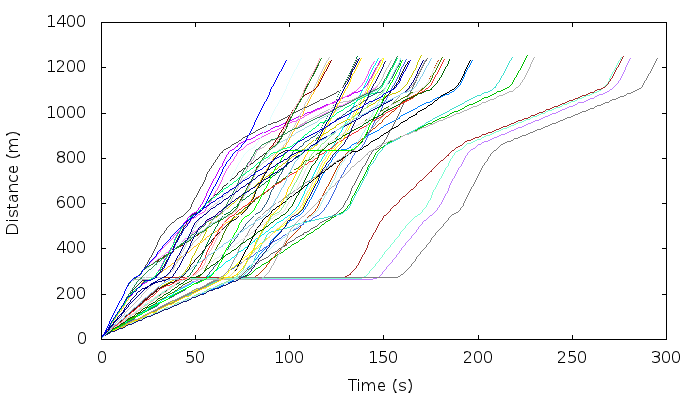
\includegraphics[width=0.5\textwidth]{images/tp0/distance100.png}
\caption{Distance graph}
\label{fig:TestResults:distance100}
\end{figure}

\subsection{Speed}
Figure~\ref{tik:speed:0:54} shows the speed at which SUMO controlled vehicles on route 54 drive as a function over time.
The graph clearly shows that the vehicles quicly accelerates up to the maximal speed, then quickly decelerates to a full stop and then quickly accelerates again.
By using \tech we see a very different outline (See Figure~\ref{fig:TestResults:speed100}).
Few vehicles decelerates to $0 m/s$, and many stay above $5 m/s$ ($18 km/h$ or $11$ miles per hour ($mph$)).
We do, however, still see a large fluctuation.
\begin{figure}[htb]
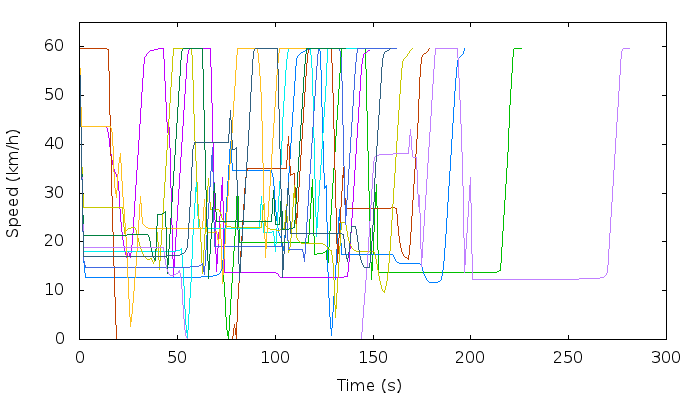
\includegraphics[width=0.5\textwidth]{images/tp0/speed100.png}
\caption{Speed graph}
\label{fig:TestResults:speed100}
\end{figure}



\subsection{Time}
It is interesting to investigate wether driving after \tech results in longer travel time than without.
It takes on average 114 seconds to drive a route in our test without \tech, and when all vehicles drive with \tech it takes 111 seconds. 
We therefore do not see any significant differens in thees results.


